\documentclass[11pt]{article}

\usepackage{adjustbox}
\usepackage{caption}
\usepackage{float}
\usepackage[T1]{fontenc}
\usepackage{graphicx}
\usepackage[utf8]{inputenc}
\usepackage{multicol}
\usepackage{multirow}
\usepackage{subcaption}
\usepackage[normalem]{ulem}
\usepackage[svgnames]{xcolor}
\usepackage[paperheight=29.69cm,paperwidth=21.01cm,left=2.54cm,right=2.54cm,top=2.54cm,bottom=2.54cm]{geometry}
\usepackage{xurl}


\setlength\parindent{0pt}
\renewcommand{\arraystretch}{1.3}



\begin{document}


\begin{center}
{\large \textbf{\textit{
\includegraphics[width=4.3cm,height=4.3cm]{./images/image4.png} }}}
\end{center}

\begin{center}
{\large \textbf{\textit{Data Science $\&$ Business Intelligence}}}
\end{center}


\begin{center}
{\large \textbf{\textit{Joel Mattsson 2024/2025}}}
\end{center}


\begin{center}
{\large \textbf{\textit{1001343}}}
\end{center}



%%%%%%%%%%%%  This Produces Table Of Contents  %%%%%%%%%%%%
\tableofcontents
\vspace{6\baselineskip}
\section{Introduction}

This section covers the main objectives and background context of this project, including the business, technical and expected objectives and outcomes.

\vspace{1\baselineskip}
\subsection{Business Objective}

The goal with this project is to develop models that partition the dataset into distinct segments or clusters, based on their similarities between features. A dataset from Kaggle is used, containing columns such as \textit{Education}, \textit{Marital\_Status}, \textit{Kidhome}, \textit{Teenhome}, \textit{Income} and \textit{Year\_Birth}: \url{https://www.kaggle.com/datasets/imakash3011/customer-personality-analysis}

To be specific, this dataset is primarily concerned with customers of a store, with further columns detailing their grocery expenditures. In the context of this project, these features are used, combined with feature engineering, to measure spending against incomes to derive behavioral insights for the formed clusters. As for the business objective, the outcomes of the implemented clustering methods will highlight distinctions between customer segments. These distinctions include not only behavioral insights but differences in preferences and tendencies, allowing for an improvement of user experience. By applying these models, customization and personalization is made possible, as customers’ tendencies are exposed. More precisely, this project aims to examine how family structure and marriage affects one’s personality. Spending patterns, parental investment and marital status are all examples of indicators of one’s personality. By reading this article, corporations can gain more understanding of how different personality traits manifest in their customers’ spending patterns and how to more effectively align with these patterns through tailored product offers or other forms of recommended offers. These meaningful insights can also be incorporated in situations other than targeted marketing campaigns. For instance, in physical stores, the framing, positioning and design can be tailored to identify with a target group with specific personality traits. Similarly, in websites, the graphical user interface and design can be optimized to maximize appeal to certain target audiences. By extension, the research question that guides this project is:

\begin{itemize}
	\item \textit{What is the correlation between personality traits and features such as marital status, parental status, income, and spending patterns, and how can these relationships inform targeted marketing and customer engagement strategies?}

\end{itemize}
\vspace{1\baselineskip}
\subsection{Hypothesis}

The hypothesis suggests that by using the baseline method, K-Means, alongside Agglomerative and Spectral Clustering, it is possible to achieve high-quality partitions of the data. These partitions highlight significant relationships between features, where the distances between them should reflect the degree of dissimilarity between clusters. Therefore, greater dissimilarity between external clusters, combined with strong similarity among data points within each cluster, represents the most favorable outcome. This structure facilitates the differentiation of data points and their respective clusters, enabling meaningful insights into the unique characteristics of each grouping. Moreover, to reach these conclusions, other techniques are needed to optimize the output. Prior to executing one of the three aforementioned clustering methods, Principal Component Analysis (PCA) will be performed on the dataset, with the expectation of reducing complexity and retaining relationships. Also, all of the included clustering methods have one common parameter \textit{K} that controls the number of partitioned clusters Thus, the Elbow Method will be applied to the PCA-transformed dataset to find its optimal value. This hypothesis was continuously evaluated throughout the development process by visualizations. After the preprocessing and removal of irrelevant features, the exploratory data analysis phase utilized visualizations of distributions for different metrics or features, as demonstrated in the ``2. Approach" section. However, as this project is about unsupervised learning with clustering, as opposed to supervised learning with classification, further measures for understanding the results are needed. Unlike classification, where a prediction is either right or wrong, clustering is evaluated based on the qualities of clusters. For this, Silhouette score was used to assess the performance of the three clustering methods. However, once the clusters are formed, additional visualizations to display their unique characteristics are required. Since only looking at the cluster formation without knowing what sets them apart won’t provide value for the business objective. Thus, the discovered underlying patterns and their segments are, in this project, interpreted thoroughly, specifically in the section ``3.2 Further Cluster Analysis (K-Means)". As a result, the hypothesis is concerned with being able to derive clear and actionable insights from what the clusters and their unique tendencies indicate. For this, features that are related to the defined business objective and research question must be targeted. Primarily \textit{Marital\_Status}, and \textit{Income} were used, and other features such as \textit{Children}, \textit{Spent} and \textit{Age} were created to allow for further analysis.

\vspace{1\baselineskip}
\section{Approach}

This section covers the manipulation and exploratory analysis of the dataset to gain a better understanding of how it can be partitioned into clusters.

\vspace{1\baselineskip}
\subsection{Data Preparation \& Exploration}

This section is concerned with the initial preparatory phases when dealing with the dataset. Data cleaning coupled with an exploratory data analysis for further understanding about the data point distributions is included. Hence, a detailed step-by-step summary is outlined, accompanied with a few plots.

\vspace{1\baselineskip}
\subsubsection{General Approach}

This section pertains to the common or general approaches applied to datasets to grasp their underlying nature. In data science, whether you are working with supervised or unsupervised learning, the first step is always to prepare, clean and understand what the dataset represents and how its features are related to one another.

\vspace{1\baselineskip}
\begin{enumerate}
	\item Import libraries: A multitude of libraries for data manipulation and visualization are needed

\end{enumerate}
\vspace{1\baselineskip}
\begin{enumerate}
	\item Load the dataset of CSV format: Retrieving a file containing data in a structured format that allows us to access data points separately

\end{enumerate}
\vspace{1\baselineskip}
\begin{enumerate}
	\item Confirm shape and structure of dataset: Make sure that the data was loaded correctly. This can be done through checking the length (the number of rows) or using the \textit{data.shape} command to inspect the number of rows and columns. Using the specified dataset, the shape \textit{(2240, 29)} is returned. Thus, over 2000 rows and as much as 29 columns

\end{enumerate}
\vspace{1\baselineskip}
\begin{enumerate}
	\item Display the head of the dataset: Use the first few instances as a reference to discover or confirm the natural structure and order of rows and columns

\end{enumerate}
\vspace{1\baselineskip}
\begin{enumerate}
	\item Show the distinct values of the column that is primarily related to the business objective and research question: By printing \textit{data["Marital\_Status"].unique} all of the possible values can be observed.

\end{enumerate}
\vspace{1\baselineskip}
\begin{enumerate}
	\item Check the number of unique categories contained in the \textit{Education} column using the command \textit{len(data["Education"].unique())}.

\end{enumerate}
\vspace{1\baselineskip}
\begin{enumerate}
	\item Store a copy of dataframe prior to applying operations and exploring the data’s distribution

\end{enumerate}
\vspace{1\baselineskip}
\begin{enumerate}
	\item Drop all the rows containing at least one NA value to avoid misleading calculations, and check the new shape of the dataset. As 2216 rows remain, we can conclude that 24 rows were effectively removed

\end{enumerate}
\vspace{1\baselineskip}
\begin{enumerate}
	\item Check the characteristics of the feature \textit{Marital\_Status}, as it’s related to the main research hypothesis and business objective. By using \textit{data["Marital\_Status"].unique} and \textit{len(data["Marital\_Status"].unique)}, we know that there are 8 distinct values.

\end{enumerate}
\vspace{1\baselineskip}
\begin{enumerate}
	\item Create demographic features based on existing features: \textit{Age}, \textit{Spent, Children} and \textit{Parental\_Status}. Based on the existing features

\end{enumerate}
\vspace{1\baselineskip}
\begin{enumerate}
	\item Update naming conventions of columns: Rearrange or rename features to make more sense and improve readability. For instance, a more intuitive name for \textit{MntWines} is \textit{Wines}.

\end{enumerate}
\vspace{1\baselineskip}
\begin{enumerate}
	\item Remove outliers that significantly deviate from the main trajectory of the data and cause a flawed representation of the actual pattern of the dataset. In particular, the columns \textit{Age} and \textit{Income} were modified

\end{enumerate}
\vspace{1\baselineskip}
\begin{enumerate}
	\item To gain further understanding of the dataset, multiple visualizations were made:

\end{enumerate}
\vspace{1\baselineskip}
\begin{enumerate}
	\item Histogram: Income-spending distribution with counts

\begin{figure}[H]
\centering
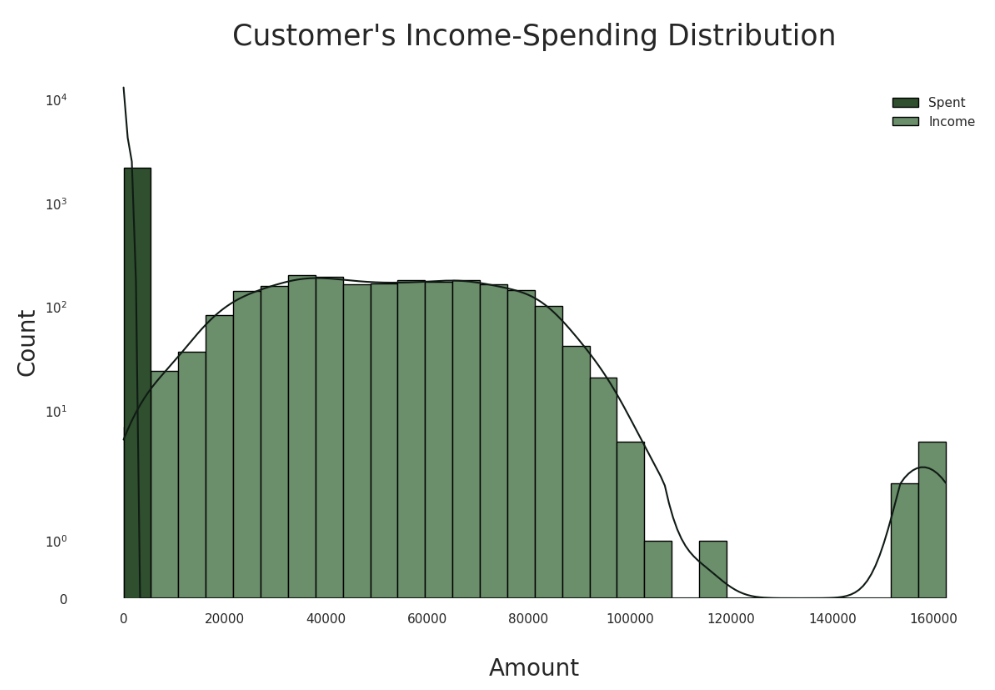
\includegraphics[width=12.7cm,height=8.83cm]{./images/image19.png}
\end{figure}


\end{enumerate}
\vspace{1\baselineskip}
\begin{enumerate}
	\item Pie chart: Education Levels of the individuals in the dataset

\end{enumerate}
\vspace{1\baselineskip}
\begin{figure}[H]
\centering
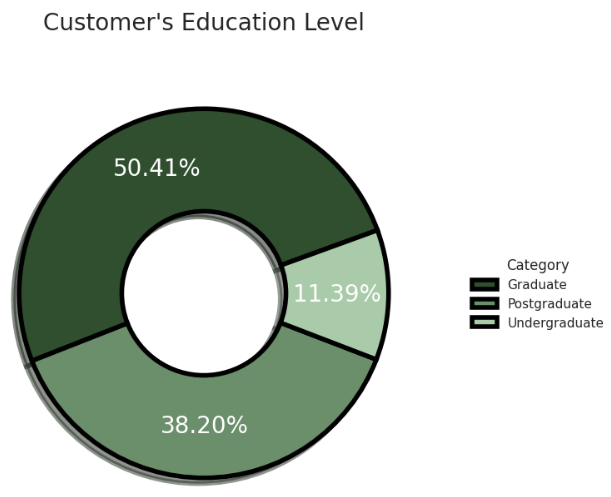
\includegraphics[width=9.52cm,height=7.73cm]{./images/image6.png}
\end{figure}


\vspace{1\baselineskip}
\begin{enumerate}
	\item Histogram: Education Level-wise income distribution

\begin{figure}[H]
\centering
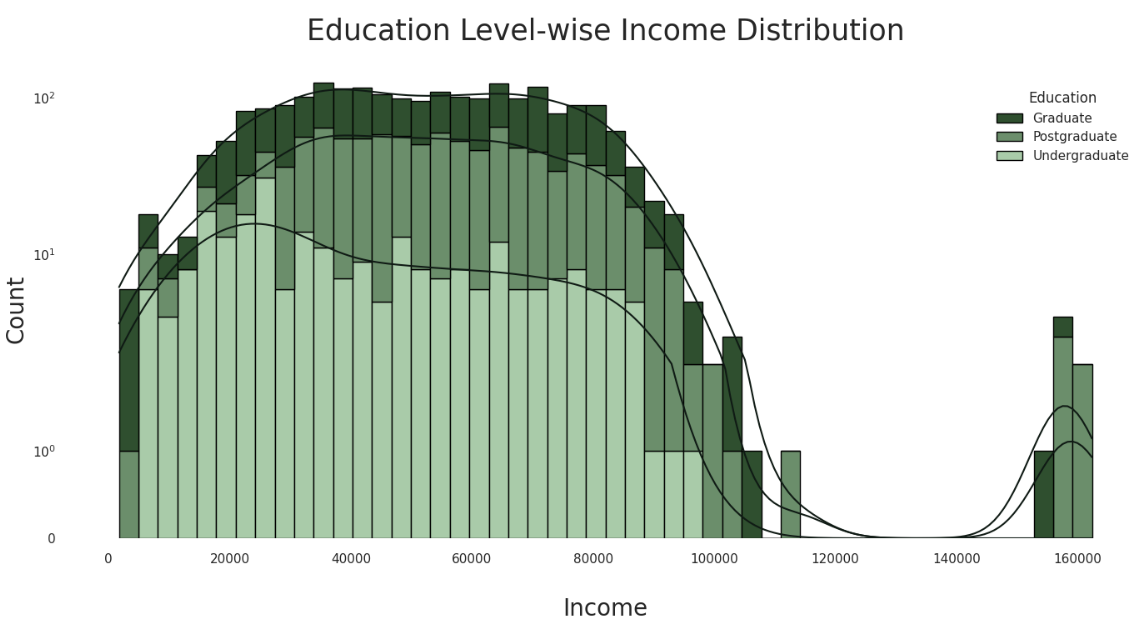
\includegraphics[width=12.9cm,height=7.11cm]{./images/image25.png}
\end{figure}


\end{enumerate}
\vspace{1\baselineskip}
\begin{enumerate}
	\item Histogram: Education Level-wise spending distribution

\begin{figure}[H]
\centering
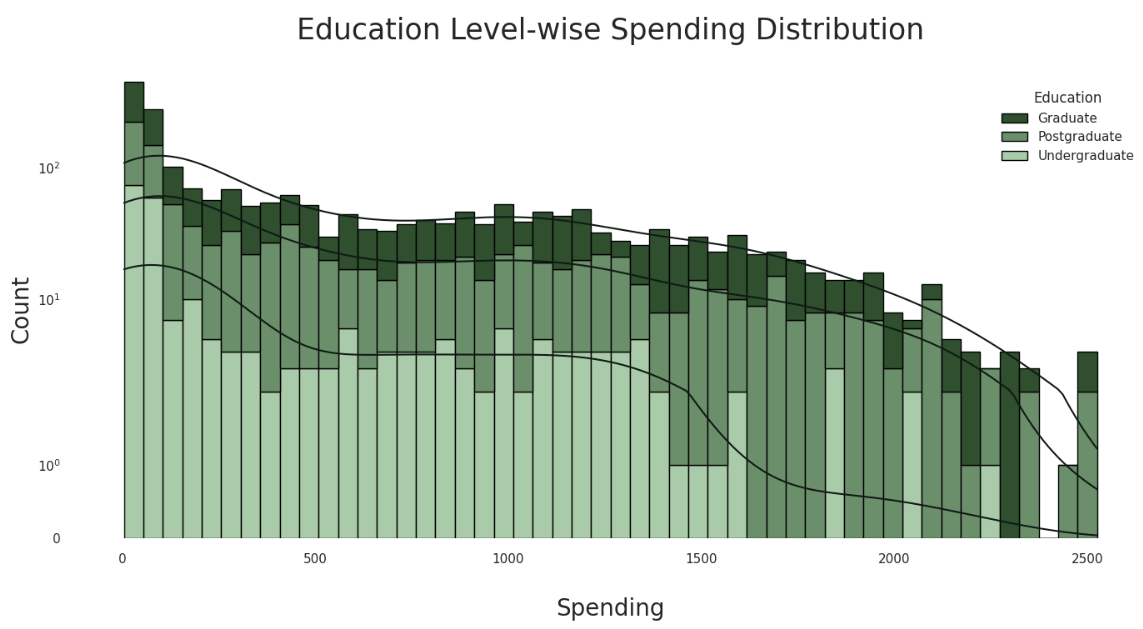
\includegraphics[width=13.16cm,height=7.24cm]{./images/image33.png}
\end{figure}


\end{enumerate}
\vspace{1\baselineskip}
\begin{enumerate}
	\item Swarm Plot: Spending distribution with Alone and Couple, where each graph checks if the individual is a parent or not

\begin{figure}[H]
\centering
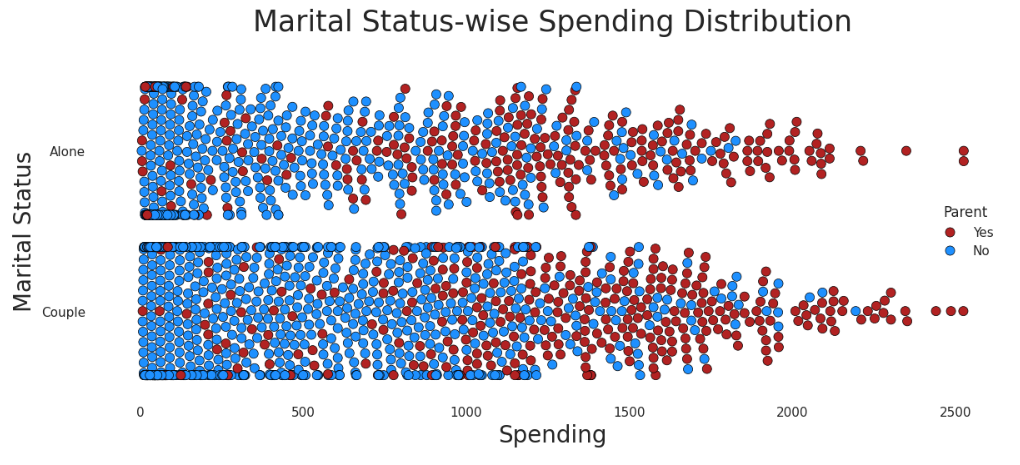
\includegraphics[width=14.24cm,height=6.52cm]{./images/image11.png}
\end{figure}


\end{enumerate}
\vspace{1\baselineskip}
\begin{enumerate}
	\item Correlation Matrix: Display the feature relationships and dependencies

\begin{figure}[H]
\centering
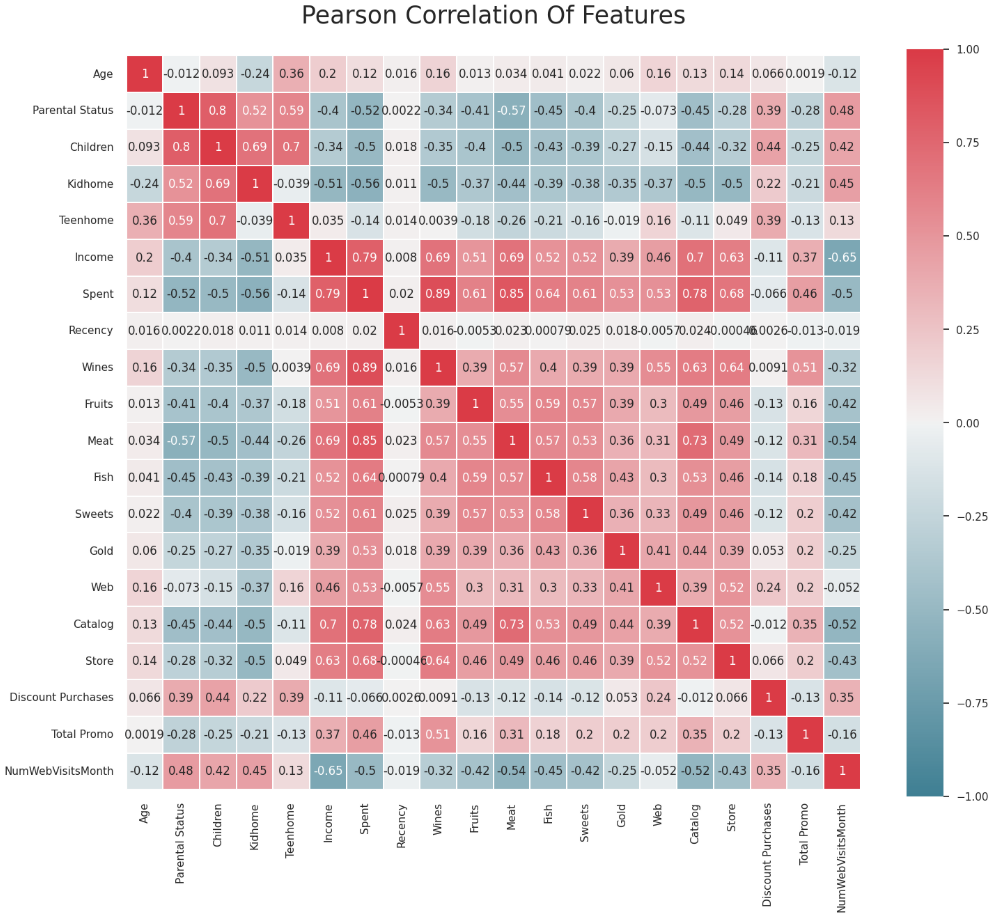
\includegraphics[width=9.67cm,height=8.9cm]{./images/image16.png}
\end{figure}


\end{enumerate}
\vspace{1\baselineskip}
\begin{enumerate}
	\item Bar chart: Show the correlation between the number of purchases and expenses

\end{enumerate}
\begin{figure}[H]
\centering
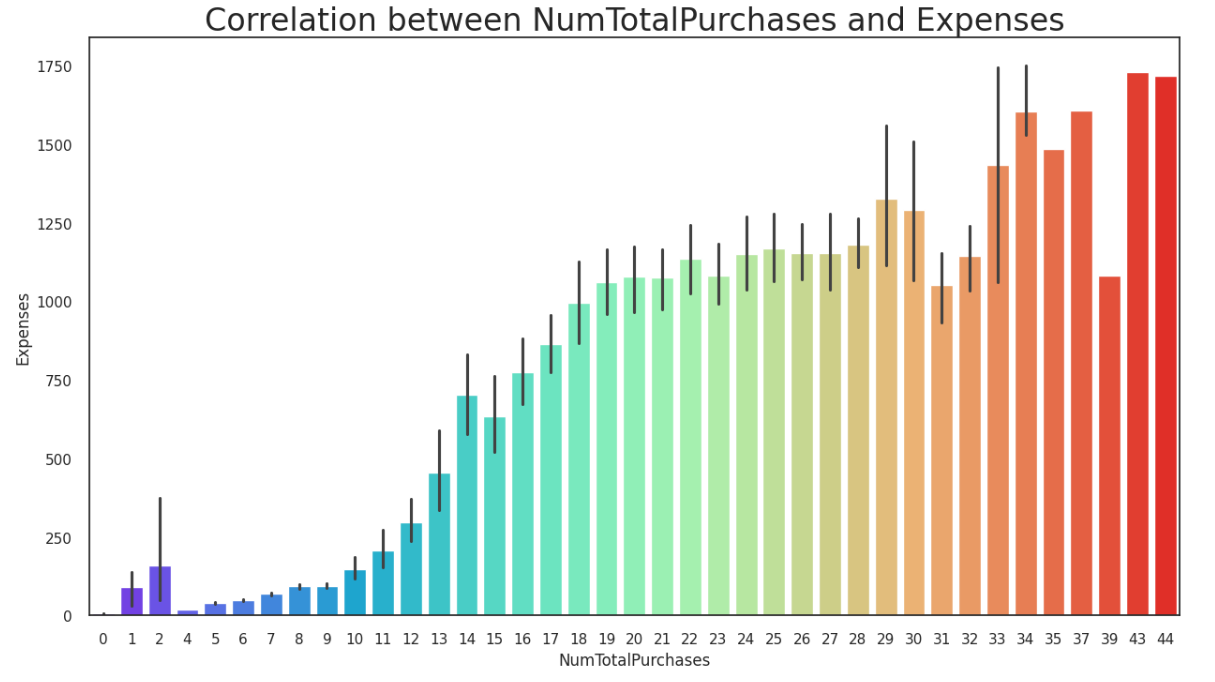
\includegraphics[width=15.47cm,height=8.66cm]{./images/image23.png}
\end{figure}


\vspace{1\baselineskip}
\subsubsection{Unsupervised Clustering Approach}

After gaining a thorough understanding of the dataset's structure and significance, the next step is to align it with the chosen branch of data science. For this project, I selected unsupervised learning with clustering. The following steps outline the process of data preparation, cleaning, and feature engineering used to implement this approach. It's important to note that these steps are carried out only after the exploratory data analysis discussed in the previous section, as understanding the data distributions is essential before clustering

\vspace{1\baselineskip}
\begin{enumerate}
	\item Drop the \textit{ID} column to facilitate the PCA transformation of feature relationships. Including redundant features only adds complexity while leaving the results unchanged

\end{enumerate}
\vspace{1\baselineskip}
\begin{enumerate}
	\item Encoding: Transform the categorial features into numerical, to increase efficiency of the PCA transformation and clustering methods. This is done through two steps:

\begin{enumerate}
	\item Get the list of contained categorical features: \textit{categorical\_features $=$ list(object\_types[object\_types].index)}

	\item Iterate through the list and use the LE object of label encoding to transform into numbers: \textit{data[i] $=$ LE.fit\_transform(data[i])}

\end{enumerate}
\end{enumerate}
\vspace{1\baselineskip}
\begin{enumerate}
	\item Standard Scaling: Use the StandardScaler class and apply it to the dataframe to scale numerical features. After printing the head of the dataframe, it appears that all values are contained in intervals where all features have the mean of 0 and a standard deviation of 1, making them easier to compare to one another

\end{enumerate}
\vspace{1\baselineskip}
\begin{enumerate}
	\item Set the number of PCA components to 3 and apply the dimensions, using the naming \textit{columns$=$(["col1","col2", "col3"])}

\end{enumerate}
\vspace{1\baselineskip}
\begin{enumerate}
	\item Visualize the reduced dimensions of the dataset when applying PCA:

\end{enumerate}
\vspace{1\baselineskip}
\begin{figure}[H]
\centering
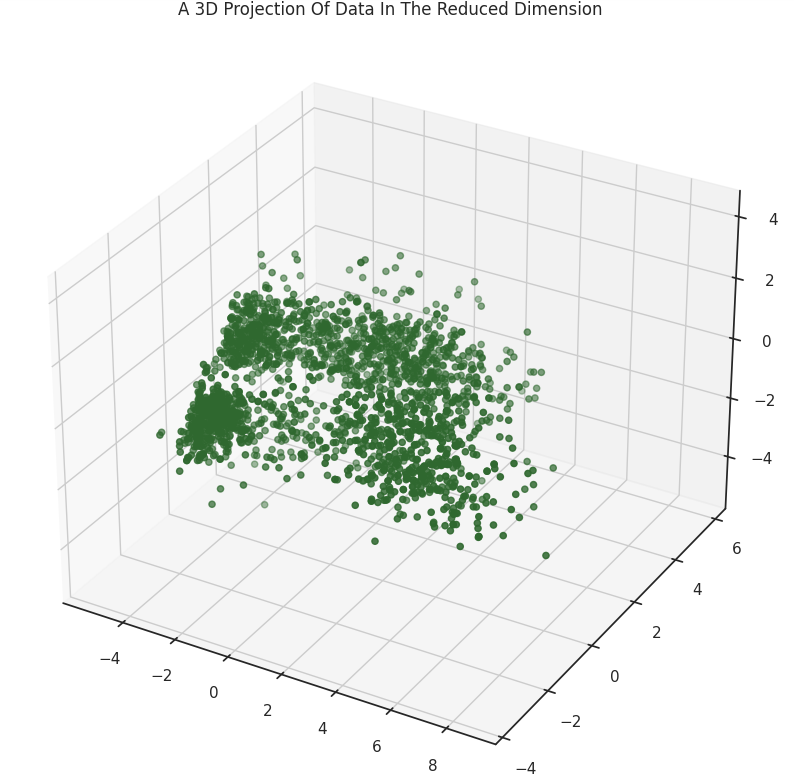
\includegraphics[width=9.26cm,height=9.11cm]{./images/image36.png}
\end{figure}


\vspace{1\baselineskip}
\begin{enumerate}
	\item Visualize the results of the Elbow Method:

\end{enumerate}
\vspace{1\baselineskip}
\begin{figure}[H]
\centering
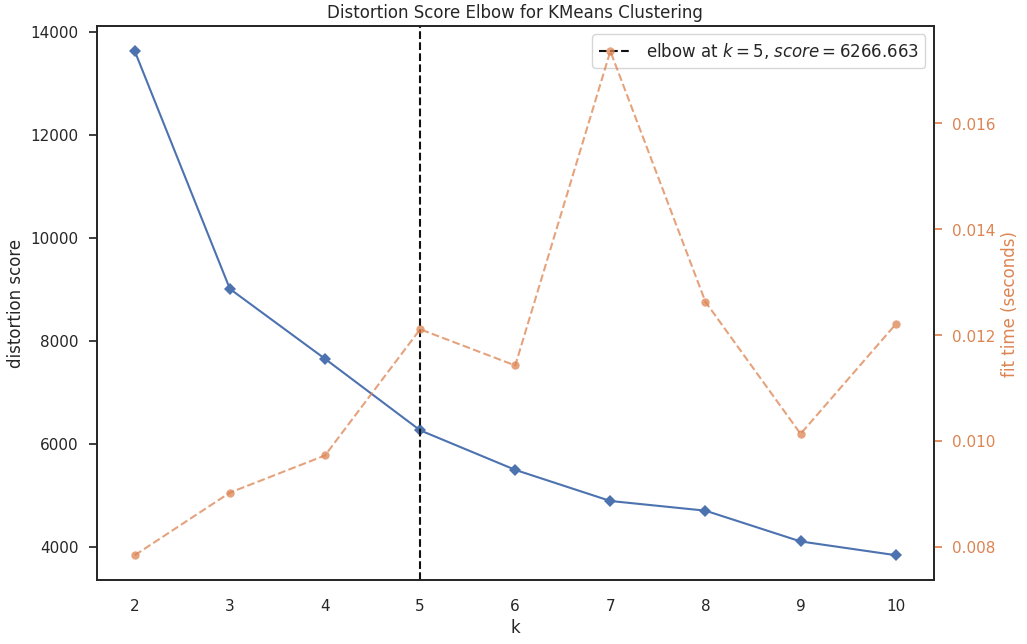
\includegraphics[width=12.21cm,height=7.66cm]{./images/image24.png}
\end{figure}


\vspace{1\baselineskip}
\subsubsection{Experienced difficulties}

In the data preparation, cleaning and exploratory data analysis, a few issues arised.

\vspace{1\baselineskip}
\begin{itemize}
	\item \textbf{Feature organization:} After exploring the dataset and examining the categorical values of the features, I encountered challenges in drawing meaningful conclusions from the provided labels. For example, the \textit{Marital\_Status} feature includes categories such as \textit{Single}, \textit{Together}, \textit{Married}, and \textit{Divorced}. To better align with the business objectives and research question, these categories can be restructured into broader groups like \textit{Alone} and \textit{Couple}. This reorganization enables the identification of more significant patterns and provides insights that add greater business value. Additionally, it allows for the visualization of stronger deviations in the data

\end{itemize}
\vspace{1\baselineskip}
\begin{itemize}
	\item \textbf{Determining the optimal number of clusters:} To determine the optimal number of clusters, I used the Elbow Method. Each clustering algorithm typically has its own unique optimal \textit{K} value for any given dataset. Consequently, implementing the Elbow Method for each clustering method would require three separate variations of the approach. Given the scope and constraints of this project, I concluded that conducting this analysis for all methods was outside the project's scope. Instead, I opted to apply the Elbow Method exclusively to the K-Means algorithm, as it is the baseline method. The Elbow Method analysis indicated that the optimal number of clusters is \textit{K$=$5}. However, as discussed in later sections of this report, the chosen number of clusters for the final analysis is \textit{K$=$4}. While this choice resulted in a slightly lower Silhouette Score compared to \textit{K$=$5}, the clusters produced at \textit{K$=$4} revealed clearer and more relatable differences in parental and marital status, income, and spending patterns. This decision aligns more closely with the defined business objectives and the research question guiding this project

\end{itemize}
\vspace{1\baselineskip}
\begin{itemize}
	\item \textbf{Preprocessing before applying PCA:} When I first attempted to apply PCA to the original dataset, I encountered errors because PCA requires numerical inputs. This is due to its reliance on the covariance matrix and eigenvalue decomposition, which can only process numerical data. To address this, I applied label encoding to convert categorical variables into numerical representations. Another essential preprocessing step is standard scaling. PCA depends on the variance of the data to determine principal components, and features with different ranges can distort the results. Without scaling, features with larger magnitudes dominate the calculations and skews the analysis. While skipping scaling may not result in compilation errors like the exclusion of label encoding, it can obscure meaningful patterns in the data

\end{itemize}
\vspace{1\baselineskip}
\subsection{Theoretical Background}

This section focuses on the theoretical foundations of the implemented techniques, excluding the coding details and results, which are covered in the section "3. Results $\&$ Conclusions." Instead, it provides textual explanations to justify the compatibility and relevance of each technique to the project’s objectives. A total of six techniques were implemented, with K-means serving as the baseline method.

\vspace{1\baselineskip}
\subsubsection{Principal Component Analysis}

Principal Component Analysis (PCA) simplifies complex datasets in data analysis and machine learning. The goal of PCA is to reduce the number of variables while keeping as much of the original information as possible. It does this by finding key patterns, called principal components, which are combinations of the original variables that explain the most variation in the data. The first component captures the most variance, and each subsequent component captures the next largest chunk of variance while staying independent of the previous ones. To perform PCA, the data is usually standardized to handle differences in scale, as covered in the section ``2.1 Data Preparation $\&$ Exploration". In this project, for instance, label encoding and standard scaler were used for this. In addition, eigenvalues and eigenvectors are used to measure the variance that each component captures. This then serves as a metric where only the components with highest variance are kept, reducing the complexity while maintaining the core structure. In this way, this technique is beneficial for noise reduction and preparing data for machine learning models.

\vspace{1\baselineskip}
\subsubsection{Elbow Method}

The Elbow Method is a simple and visual way to figure out the best number of clusters to use in a dataset when working with clustering algorithms. In this project, the common parameter for the three implemented clustering methods is \textit{K}, representing the number of clusters to output. The idea is to strike a balance between keeping clusters meaningful and not overcomplicating things by having too many clusters. Within-cluster variance, measured as the within-cluster sum of squares (WCSS), shows how tightly grouped the points in each cluster are. The lower the value, the better, as higher intra-clustering quality is achieved. In application, the Elbow Method runs the clustering algorithm multiple times with different values for \textit{K}. For each execution, a WCSS score is calculated and used as the y-value and plotted with the associated value for K. The "elbow" in the graph is the point where the WCSS stops dropping steeply, suggesting that adding more clusters doesn't yield substantial improvement. This point is your sweet spot for \textit{K}, offering a good balance between simplicity and accuracy.

\vspace{1\baselineskip}
\subsubsection{K-Means Clustering}

K-Means clustering is a straightforward and popular algorithm for grouping data into \textit{K} clusters based on similarities. The goal is to ensure points within each cluster are more similar to each other than to points in other clusters. This is made possible with an iterative approach: First, the algorithm randomly selects K cluster centers, denoted as centroids. Then, it iteratively alternates between two steps:

\begin{enumerate}
	\item Assign each data point to the nearest centroid

	\item Recalculate the centroids by finding the average position of the points assigned to each cluster

\end{enumerate}
\vspace{1\baselineskip}
This process repeats until the centroids stop moving, or a maximum number of iterations is reached. Ideally, centroids with negligible movement indicate consistently identified clusters, ensuring high intra-cluster similarity and low inter-cluster similarity. However, K-Means has limitations. It assumes clusters are spherical and of similar size, which can make it less effective for irregular or overlapping clusters. Additionally, the algorithm is sensitive to the initial placement of centroids, potentially leading to different results across runs. Poor initialization may also cause the algorithm to get stuck in a local optimum. Despite these challenges, K-Means offers several benefits. It is computationally efficient, making it well-suited for large datasets. It’s also easy to understand and implement, making it a great starting point for clustering tasks. K-Means works effectively in many practical scenarios, such as customer segmentation, and anomaly detection, making it a versatile and valuable approach.

\vspace{1\baselineskip}
\subsubsection{Agglomerative Clustering}

Agglomerative clustering is a hierarchical method used to group data points by building a nested hierarchy of clusters based on their similarity. The process begins with each data point as its own cluster, and the algorithm iteratively merges the two most similar clusters until either all points are combined into a single cluster or a desired number of clusters is achieved. The proximity between clusters is determined using different linkage criteria, such as single linkage (minimum distance), complete linkage (maximum distance), or average linkage (mean distance). These linkage methods significantly affect the shape and structure of the resulting clusters. The clustering process is visualized using a tree-like diagram that shows all of the merging steps denoted as a dendrogram. Agglomerative clustering is well-suited for datasets with hierarchical relationships or non-spherical clusters, as it doesn’t assume a specific cluster shape. However, it can be computationally expensive for large datasets due to the need for pairwise distance calculations or linkages. Despite this limitation, it remains a powerful and flexible tool for analyzing smaller datasets or exploring complex data structures.

\vspace{1\baselineskip}
\subsubsection{Spectral Clustering}

Spectral clustering is a powerful and adaptable algorithm that leverages graph theory and eigenvalue decomposition to group data points based on their relationships or similarities. Unlike K-Means, it’s well-suited for identifying clusters with complex or irregular structures beyond simple spheres. The process begins by representing the data as a graph, where each point is a node and edges indicate similarities, often derived from a similarity matrix or nearest-neighbor relationships. A critical step involves constructing the Laplacian matrix from the graph and calculating its eigenvalues and eigenvectors. These eigenvectors enable the transformation of data into a lower-dimensional space. Clusters are then identified by applying a standard algorithm like K-Means to this transformed representation. Conclusively, while Spectral Clustering is effective for handling underlying patterns, it can be computationally expensive for large datasets due to the eigen calculations.

\vspace{1\baselineskip}
\subsubsection{Silhouette Score}

The Silhouette Score is a widely used metric for evaluating the quality of clustering by assessing how well data points fit within their assigned clusters. Its primary role is to measure the compactness of clusters and their separation from one another, making it useful for determining the optimal number of clusters or comparing different clustering methods. For each data point, the score is calculated using the formula:

\begin{figure}[H]
\centering
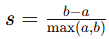
\includegraphics[width=2.61cm,height=0.91cm]{./images/image17.png}
\end{figure}


\textit{Where..}

\begin{itemize}
	\item \textit{\textbf{a} is the average distance to other points within the same cluster (intra-cluster distance)}

	\item \textit{\textbf{b} is the average distance to points in the nearest neighboring cluster (inter-cluster distance)}

\end{itemize}
\vspace{1\baselineskip}
The Silhouette Score ranges from -1 to 1, with values close to 1 indicating that the point is well-suited to its cluster and poorly aligned with others. Scores near 0 suggest overlapping clusters, while negative values indicate potential misclassification. The overall score is the mean of all data points' scores in the dataset. This metric is particularly valuable for unsupervised clustering algorithms since it provides an intuitive measure of clustering quality without relying on ground truth labels. However, calculating the score can be computationally demanding for large datasets, as it requires computations for all data points.

\vspace{1\baselineskip}
\section{Results \& Conclusions}

This section covers insights and meaningful conclusions derived from the visualizations grouped by clusters. The textual description of each plot is followed below the pictures, where one or more of the bullet points \textit{Insights}, \textit{Conclusions} and \textit{Background Information} are presented. As for \textit{Background Information}, this mark is only added for visualizations that require more context to understand the connection to the defined business objective.

\vspace{1\baselineskip}
\subsection{Multiple Cluster Method Comparison}

Below, a few visual illustrations that compare all of the three clustering methods and their respective performances are shown. Note that this section is limited to the overall cluster formations.

\vspace{1\baselineskip}
\begin{figure}[H]
\centering
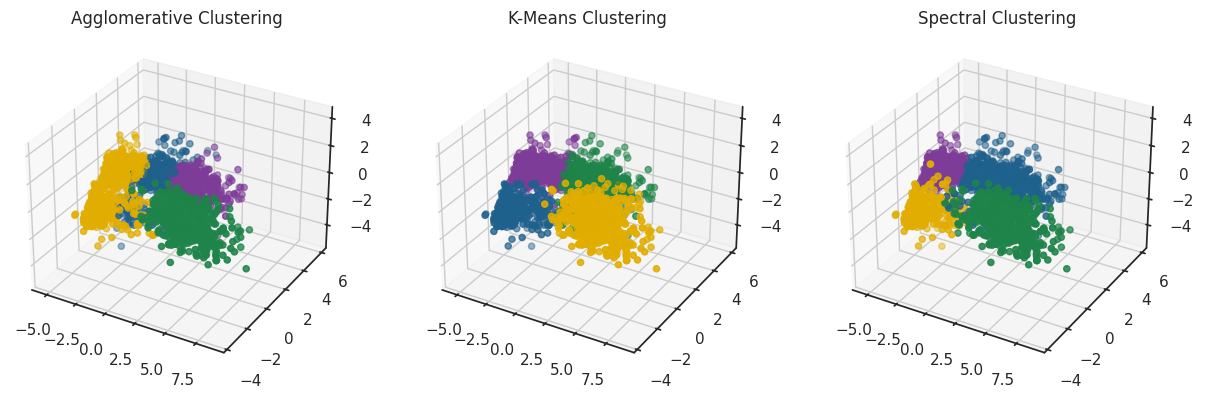
\includegraphics[width=15.92cm,height=5.33cm]{./images/image13.png}
\end{figure}


\vspace{1\baselineskip}
\begin{itemize}
	\item \textbf{Insights:} Each clustering method has different outcomes, yet they are quite similar in their partitioning, such that similar characteristics of the groups can be spotted. Thus, their cluster performance, or silhouette scores can be expected to be similar

\end{itemize}
\vspace{1\baselineskip}
\begin{itemize}
	\item \textbf{Conclusions:} Despite the differences of algorithmic approaches for each method, they produce relatively similar results for the particular dataset in this project. For Agglomerative, K-Means and Spectral Clustering, the parameter that is common for all is \textit{K}. In essence, this parameter allows developers to adjust the number of clusters that the method produces. In this way, the depth or thoroughness that the method has to perform in its analysis of clusters is regulated. A higher value for \textit{K} suggests that a more detailed search of feature discrepancies and relationships has to be conducted, as each data partition must be distinguished into separate clusters by their qualities. Conversely, lower values for \textit{K} entail a more simple division of data points, where only the most prominent feature relationships that are easy to locate divides the few clusters. Thus, the very parameter \textit{K} bridges the Agglomerative, K-Means and Spectral Clustering, which, as the visualization above illustrates, results in cases where their performances are similar if their configured \textit{K} values are identical. Conclusively, \textit{K} serves as the common denominator for these methods, making them applicable to problems of similar nature.

\end{itemize}
\vspace{1\baselineskip}
\begin{figure}[H]
\raggedright
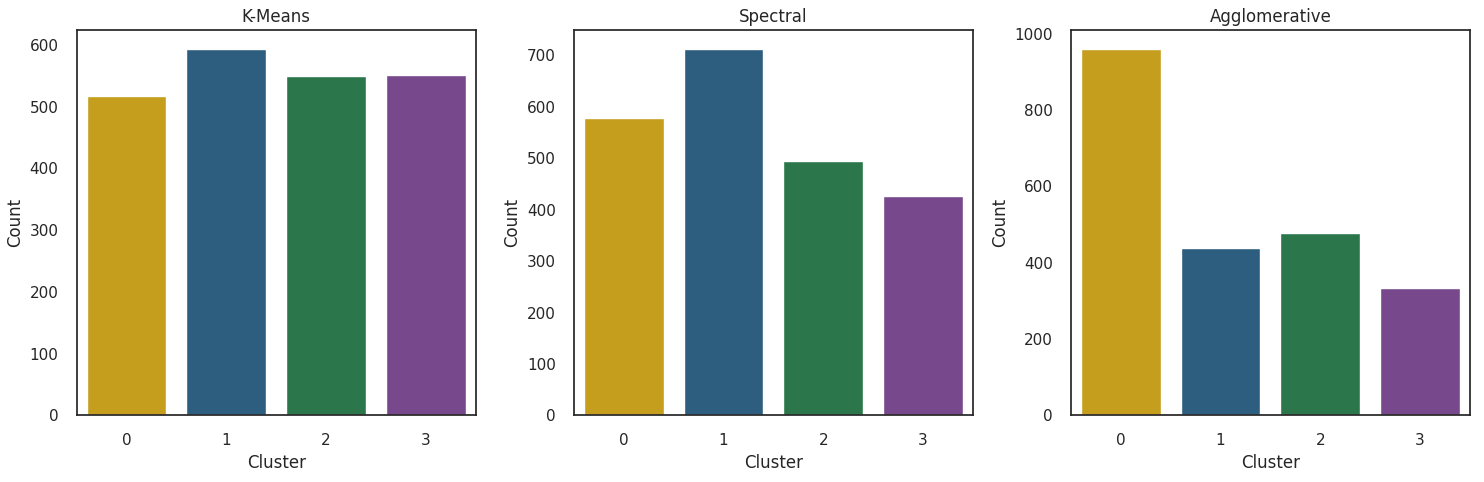
\includegraphics[width=15.92cm,height=5.19cm]{./images/image29.png}
\end{figure}


\begin{itemize}
	\item \textbf{Insights:} Considering the previous clustering visualizations, these bar charts make sense. Both visualizations indicate a strong similarity and partitioning of data. However, the distributions are slightly distinguished, especially for Agglomerative Clustering

\end{itemize}
\vspace{1\baselineskip}
\begin{itemize}
	\item \textbf{Conclusions:} Each clustering method partitions the data uniquely as expected. The distributions of K-Means and Spectral Clustering are more similar than Agglomerative, but all methods are applicable to the dataset

\end{itemize}
\vspace{1\baselineskip}
\begin{figure}[H]
\centering
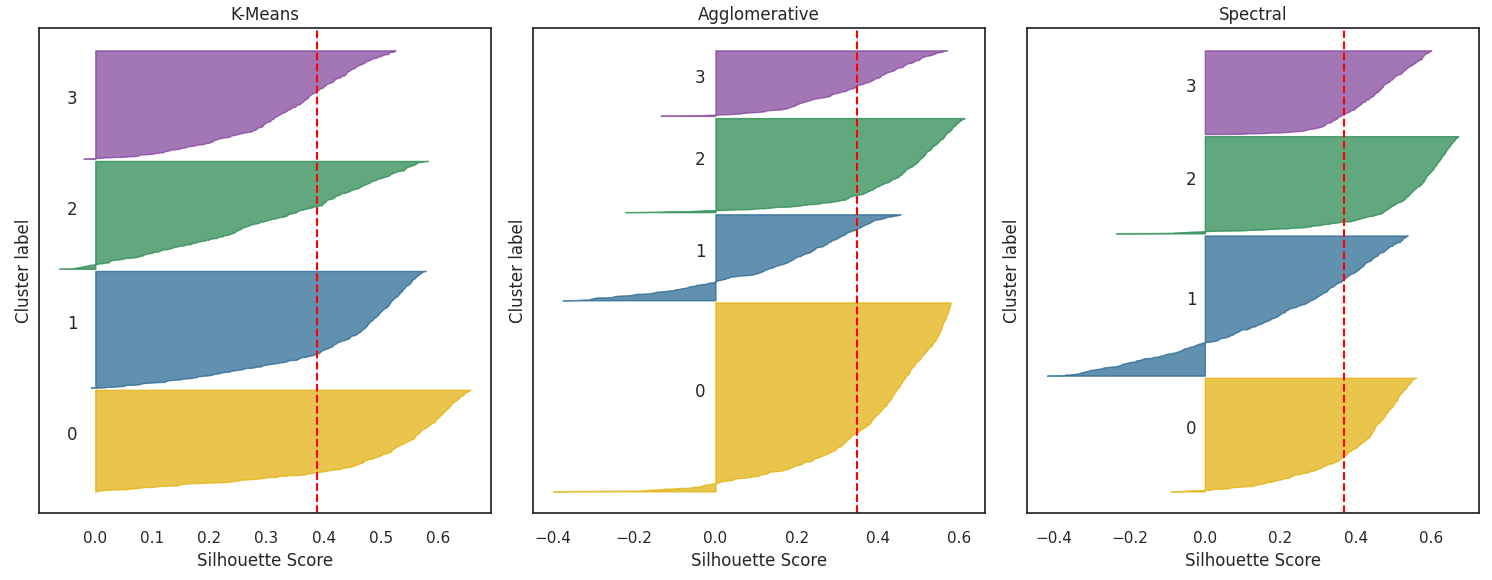
\includegraphics[width=15.92cm,height=6.17cm]{./images/image21.png}
\end{figure}


\begin{figure}[H]
\centering
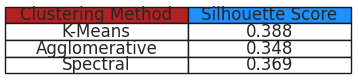
\includegraphics[width=8.46cm,height=1.89cm]{./images/image2.png}
\end{figure}

\vspace{1\baselineskip}


\begin{itemize}
	\item \textbf{Insights:}

\begin{itemize}
	\item The Silhouette Score for Agglomerative Clustering is slightly worse than the two other methods. By only observing their average scores and discrepancy in partitioning of data for the clusters, this can be identified
        \item K-Means and Spectral Clustering appears to be more suitable choices, given the context of this project with respect to the selected dataset. Besides their appropriate partitioning, as derived not only from the table above but from the two previous ones, their silhouette scores are also more consistent

\end{itemize}
\end{itemize}

\vspace{1\baselineskip}
\begin{itemize}
	\item \textbf{Conclusions:} As the previous bar charts indicate, Agglomerative Clustering appears to have a more skewed division of the clusters, resulting in a lower SIlhouette score. Nevertheless, all methods yield satisfying results, considering the range of evaluation is [-1, 1]. This entails that, in percentage, K-Means, Spectral and Agglomerative equates to 69.4$\%$, 68.45$\%$ and 67.4$\%$ respectively.

\end{itemize}
\vspace{1\baselineskip}
\subsection{Further Cluster Analysis of The Baseline Method}

This section is related to the results of the selected baseline method. In the report for this project, I opted for K-Means. However, as can be seen in the Python notebook, the developer can freely switch between the three implemented clustering methods as the baseline. As such, the results demonstrated in this section can be replicated with roughly the same outcomes and visualizations for Agglomerative and Spectral Clustering. More information on this is covered in the section ``5.1 Baseline Method Selection".

\vspace{1\baselineskip}
\begin{figure}[H]
\centering
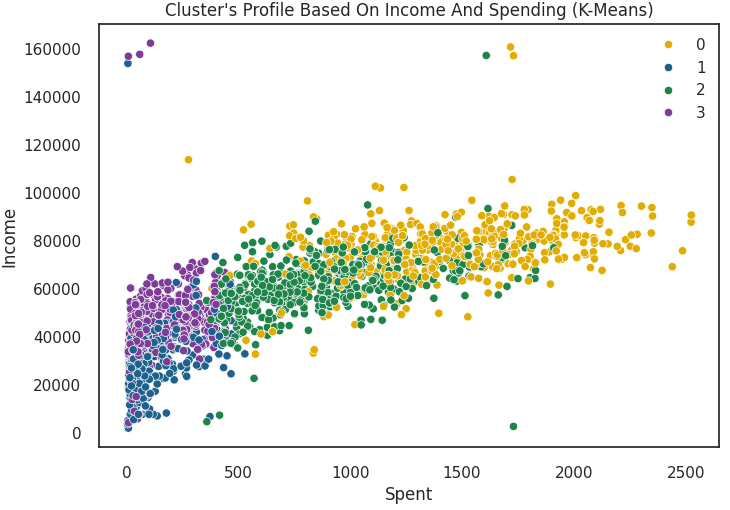
\includegraphics[width=11.35cm,height=7.9cm]{./images/image3.png}
\end{figure}


\begin{itemize}
	\item \textbf{Insights:}

\begin{itemize}
	\item \uline{\textcolor[HTML]{BF9000}{Cluster 0:}} High income $\&$ High spending

	\item \uline{\textcolor[HTML]{0B5394}{Cluster 1:}} Low income $\&$ Low spending

	\item \uline{\textcolor[HTML]{38761D}{Cluster 2:}} High income $\&$ Average spending

	\item \uline{\textcolor[HTML]{674EA7}{Cluster 3:}} Low income $\&$ Low spending

\end{itemize}
\end{itemize}
\vspace{1\baselineskip}
\begin{itemize}
	\item \textbf{Conclusions:} The chart demonstrates a strong distinction of tendencies for the clusters, where the colored data points are grouped accordingly. Using the visualization above, we can conclude that income levels are clearly a prominent factor that contribute to each of the segments. First of all, before diving into the behavioral implications of each cluster, it’s important to recognize the overall pattern that applies to the broader population. It appears that, in general, as the income increases, the spending also increases. However, the higher the income, the less the spending tends to increase. This results in an exponential curve, where a steep upward curve is characterized for \uline{\textcolor[HTML]{0B5394}{Cluster 1}} and \uline{\textcolor[HTML]{674EA7}{Cluster 3}}, the ones with the least income. The rise of the curve becomes less sharp for \uline{\textcolor[HTML]{38761D}{Cluster 2}}, and finally, a plateau is reached for \uline{\textcolor[HTML]{BF9000}{Cluster 0}}, the most affluent group

\end{itemize}
\vspace{2\baselineskip}
\begin{figure}[H]
\centering
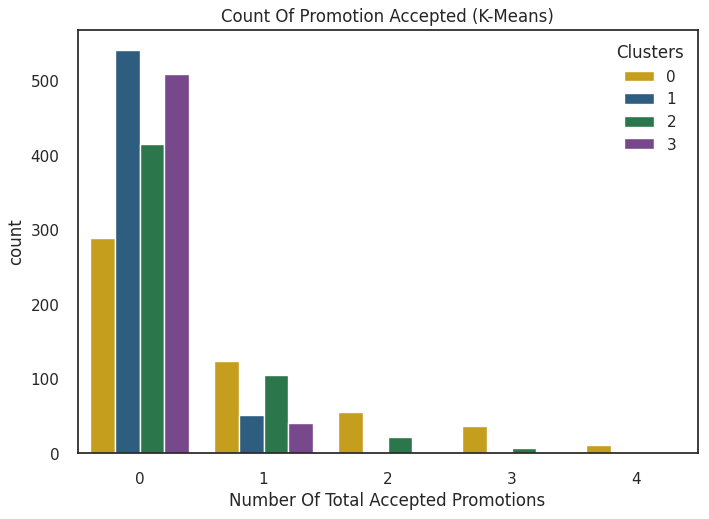
\includegraphics[width=10.86cm,height=7.94cm]{./images/image34.png}
\end{figure}


\vspace{1\baselineskip}
\begin{itemize}
	\item \textbf{Insights:}

\begin{itemize}
	\item \uline{\textcolor[HTML]{BF9000}{Cluster 0}}, the yellow, has the highest income as indicated by the last chart. In this bar chart, it appears that individuals in this cluster accepts more promotions as well

	\item \uline{\textcolor[HTML]{0B5394}{Cluster 1}} and \uline{\textcolor[HTML]{674EA7}{Cluster 3}}, which the previous chart established as individuals with lower incomes, only receive 0 or 1 promotions. This is reasonable since there's a correlation between income and the number of consumption-promotions

	\item \uline{\textcolor[HTML]{38761D}{Cluster 2}}, previously established as high income with average spending, also has a greater number of accepted promotions

\end{itemize}
\end{itemize}
\vspace{1\baselineskip}
\begin{itemize}
	\item \textbf{Conclusions:} This bar chart builds on the insights from the previous chart, which highlighted income and spending patterns, by emphasizing that income is closely linked to the number of promotions received and accepted throughout a career. This conclusion is supported by the strong alignment observed in each cluster between levels of income and the number of promotions, illustrating a clear pairwise relationship and direct correlation.

\end{itemize}
\vspace{2\baselineskip}
\begin{figure}[H]
\centering
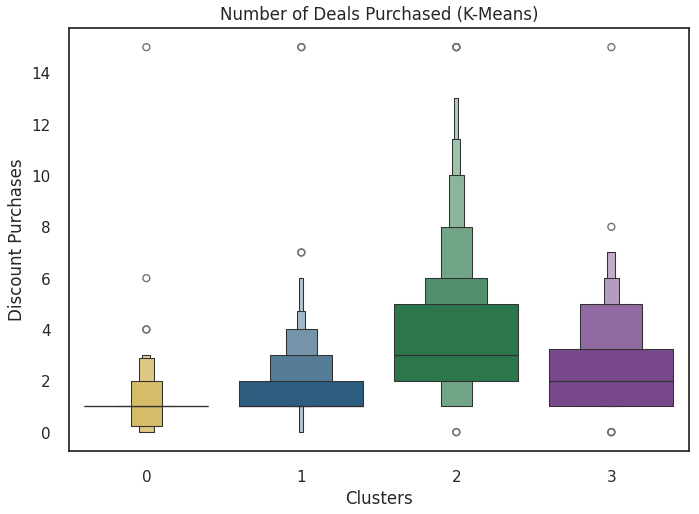
\includegraphics[width=10.67cm,height=7.85cm]{./images/image15.png}
\end{figure}


\begin{itemize}
	\item \textbf{Background information:} The attribute representing the number of deals purchased may be confusing to grasp in the context of the defined business objective. In essence, these deals are derived from the specific retail grocery store to which the dataset pertains. These deals are specifically focused on family-related matters, designed for kids, teenagers, and young adults. Therefore, the target audience is the newest generation, making parents the primary marketing focus. By extension, insights into the connection between parental status, marital status, and personality traits can be observed, highlighting their relevance to the defined business objective

\end{itemize}
\vspace{1\baselineskip}
\begin{itemize}
	\item \textbf{Insights:}

\begin{itemize}
	\item It turns out that, despite the high spending of \uline{\textcolor[HTML]{BF9000}{Cluster 0}}, it isn't into product deals offered by the store

	\item \uline{\textcolor[HTML]{38761D}{Cluster 2}}, with the second highest income, invest the most financial resources on discount deals

\end{itemize}
\end{itemize}
\vspace{1\baselineskip}
\begin{itemize}
	\item \textbf{Conclusions:} \uline{\textcolor[HTML]{0B5394}{Cluster 1}}, \uline{\textcolor[HTML]{38761D}{Cluster 2}} and \uline{\textcolor[HTML]{674EA7}{Cluster 3}} find the product offers more appealing. Although \uline{\textcolor[HTML]{38761D}{Cluster 2}} spends most on deals by far, it’s important to look at the chart through the lens of disposable income. As established in a previous chart, income and spendings are highly correlated, and \uline{\textcolor[HTML]{38761D}{Cluster 2}} has a significantly higher income than its two adjacent clusters. As a result, assuming these three clusters have equal interest levels in purchasing deals, \uline{\textcolor[HTML]{38761D}{Cluster 2}} will naturally invest more financial resources. For that reason, the visualization cannot be purely interpreted by what it shows. By accounting for correlations that previous charts suggest, the plot reveals an interesting pattern. Considering that these deals are targeted toward families, we can conclude that \uline{\textcolor[HTML]{BF9000}{Cluster 0}} has no interest in becoming parents. At first glance, \uline{\textcolor[HTML]{38761D}{Cluster 2}} seems to show the greatest interest in having children. However, taking into account the low incomes of \uline{\textcolor[HTML]{0B5394}{Cluster 1}} and \uline{\textcolor[HTML]{674EA7}{Cluster 3}}, combined with their significant financial investment in family-oriented discount deals, it suggests that these groups frequently become parents. Ultimately, \uline{\textcolor[HTML]{674EA7}{Cluster 3}} demonstrates a slightly stronger inclination toward starting a family, as it represents the lowest income group yet allocates a larger portion of its spending to these deals

\end{itemize}
\vspace{2\baselineskip}
\begin{figure}[H]
\centering
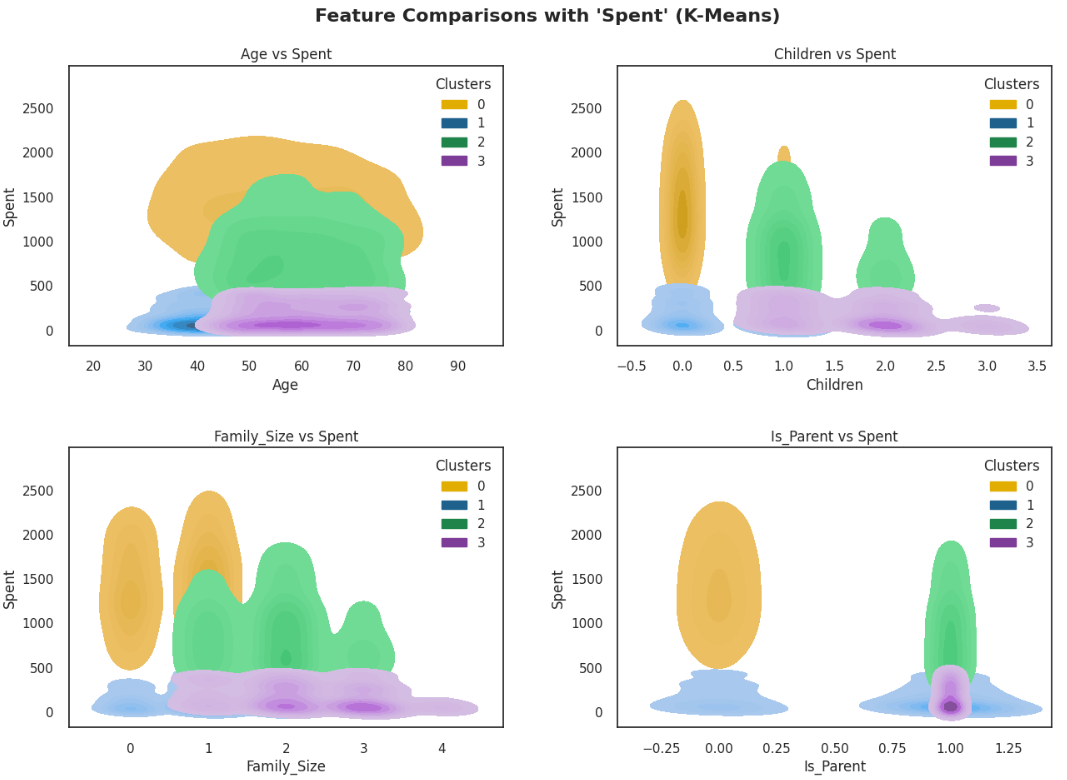
\includegraphics[width=14.81cm,height=10.85cm]{./images/image1.png}
\end{figure}


\vspace{1\baselineskip}
\begin{itemize}
	\item \textbf{Background information:} In the sub-plot in the bottom right corner, \textit{Is\_Parent} represents a boolean, where 0 maps to \textit{False} and 1 indicates \textit{True}

\end{itemize}
\vspace{1\baselineskip}
\begin{itemize}
	\item \textbf{Insights:}

\begin{itemize}
	\item \textbf{Age vs Spent:} For the two clusters with the highest incomes (Cluster 0 and 2), the peak years of spending lies between ages 40-50, and then it slowly reduces as the individuals get older. However, the spending is low throughout ages 25-80 for the two remaining clusters with lower income

	\item \textbf{Family\_Size vs Spent $\&$ Children vs Spent:} Both diagrams indicate that \uline{\textcolor[HTML]{BF9000}{Cluster 0}}, having the highest income, also preferably have smaller families but simultaneously spend more. Conversely, \uline{\textcolor[HTML]{0B5394}{Cluster 1}} and \uline{\textcolor[HTML]{674EA7}{Cluster 3}}, with lower incomes, have more kids and larger families. \uline{\textcolor[HTML]{38761D}{Cluster 2}} is in the middle of these two extremes

	\item \textbf{Is\_Parent vs Spent:} \uline{\textcolor[HTML]{BF9000}{Cluster 0}} is not interested in becoming parents at all, whereas \uline{\textcolor[HTML]{38761D}{Cluster 2}} and \uline{\textcolor[HTML]{674EA7}{Cluster 3}} are very interested in parental investment. \uline{\textcolor[HTML]{0B5394}{Cluster 1}} is divided on this issue, such that some become parents and others not

\end{itemize}
\end{itemize}
\vspace{1\baselineskip}

\begin{itemize}
	\item \textbf{Conclusions:}

\begin{itemize}
	\item \textbf{Age vs Spent:} First of all, the chart with \textit{Age} and \textit{Spent} highlights a pattern for the two more economically affluent clusters (0 and 2), where the peak years of spending lie between ages 40-50. Thus, these individuals dedicate their young-adult-years (20-30) to building a career, and once they reach 40 and have accumulated wealth and safety, their expenditures on leisure tend to increase. However, this spending gradually decreases as their retirement years approach. Conversely, the other two clusters (1 and 3) that are operating with less disposable income, are consistently maintaining their low level of spending for all ages. This is a consequence of their low income level that holds them back from spending more money on leisure and luxuries for amusement and comfortability. Their strategy then translates into a balance between a few luxuries and keeping up with necessities such as housing and kids. In other words, their investment in luxuries is continuous but restricted to a low level

    \item \textbf{Family\_Size vs Spent $\&$ Children vs Spent:} These two subplots primarily indicate that economic status doesn’t necessarily influence one’s choice of becoming a parent. In this way, the common stereotype where couples avoid having kids solely because of money issues is refuted. Thus, parental status has more to do with one’s personality and core values. Two contrasting extremes in this case would be:

\begin{itemize}
	\item \textit{Prioritizing family to the point that personal freedom and flexibility is restrained}

	\item \textit{Neglecting family to gain more economic freedom and time on one’s own terms}

\end{itemize}


\end{itemize}
\end{itemize}


In the visualization above, it appears that \uline{\textcolor[HTML]{BF9000}{Cluster 0}} has core values more concerned with personal freedom and flexibility, whereas \uline{\textcolor[HTML]{674EA7}{Cluster 3}} advocates for big families despite their suboptimal economic conditions. \uline{\textcolor[HTML]{0B5394}{Cluster 1}} and \uline{\textcolor[HTML]{38761D}{Cluster 2}} are more in the middle of these two extremes. The first one switches between having children or remaining child-free, and if they decide to have kids, it only ranges between 1 and 2. The latter one is in a better economic situation and consistently chooses to have children, but not as many as \uline{\textcolor[HTML]{674EA7}{Cluster 3}}, implying that they also value freedom and privacy like \uline{\textcolor[HTML]{BF9000}{Cluster 0}}

	\textbf{Is\_Parent vs Spent:} As highlighted in the previous boxplot chart, \uline{\textcolor[HTML]{BF9000}{Cluster 0}} avoids discount deals by virtue of their lack of interest in becoming parents. \uline{\textcolor[HTML]{1155CC}{Cluster 1}}, which was the second most resistant to deals in the previous chart, is also the second most resistant to becoming a parent, where a clear division of opinions on parenting is illustrated. In this chart, \uline{\textcolor[HTML]{38761D}{Cluster 2}} and \uline{\textcolor[HTML]{674EA7}{Cluster 3}} appears to have similar interests in becoming or being parents, where spendings is the only factor distinguishing them

\vspace{6\baselineskip}
\begin{figure}[H]
\centering
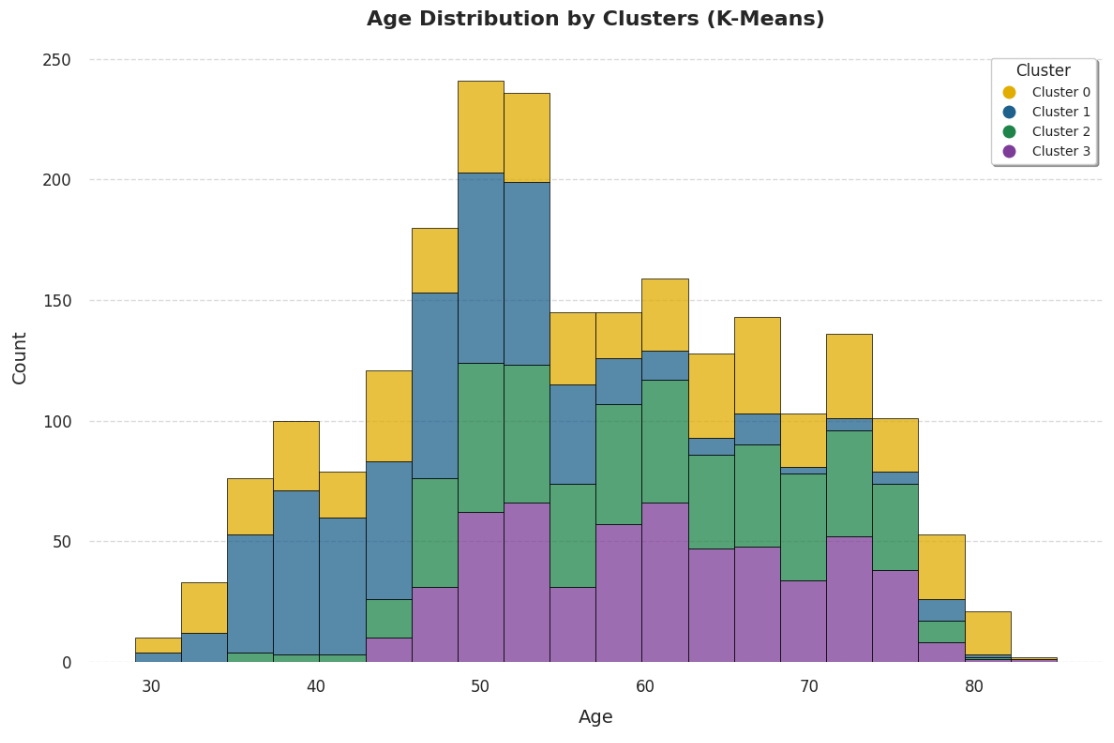
\includegraphics[width=13.99cm,height=9.3cm]{./images/image12.png}
\end{figure}


\vspace{1\baselineskip}
\begin{itemize}
	\item \textbf{Insights:}

\end{itemize}
\begin{itemize}
	\item \uline{\textcolor[HTML]{BF9000}{Cluster 0:}} Uniform distribution across age 30-80

	\item \uline{\textcolor[HTML]{0B5394}{Cluster 1:}} Primarily between 35-55

	\item \uline{\textcolor[HTML]{38761D}{Cluster 2:}} Concentrated on ages in the range of 50-75

	\item \uline{\textcolor[HTML]{674EA7}{Cluster 3:}} Most are 50-80 years old

\end{itemize}
\vspace{1\baselineskip}
\begin{itemize}
	\item \textbf{Conclusions:} The age distributions for \uline{\textcolor[HTML]{BF9000}{Cluster 0}} and \uline{\textcolor[HTML]{0B5394}{Cluster 1}} are the closest to an even distribution, whereas \uline{\textcolor[HTML]{38761D}{Cluster 2}} and \uline{\textcolor[HTML]{674EA7}{Cluster 3}} consist exclusively of older individuals. Referring to previous charts that suggest \uline{\textcolor[HTML]{38761D}{Cluster 2}} and \uline{\textcolor[HTML]{674EA7}{Cluster 3}} are statistically the most likely to start a family and have children, they also appear to be the two clusters with the oldest age groups. This suggests that, in general, as people grow older, they tend to place greater value on family

\end{itemize}
\vspace{2\baselineskip}
\begin{figure}[H]
\centering
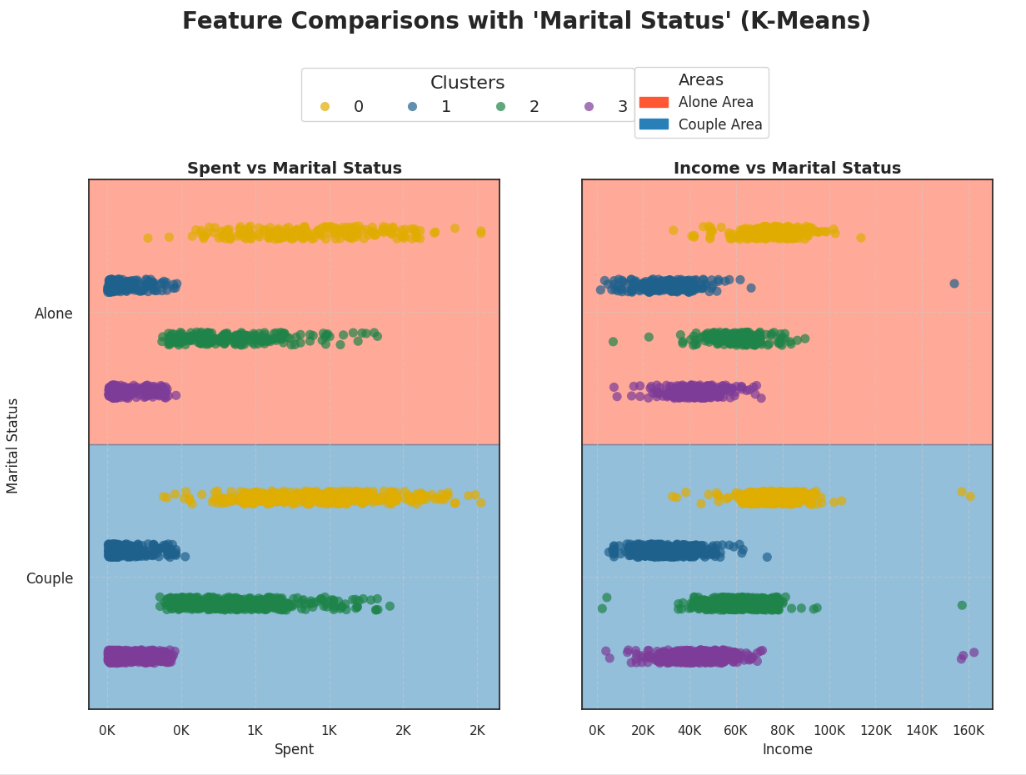
\includegraphics[width=13.33cm,height=10.12cm]{./images/image32.png}
\end{figure}


\textbf{Insights:}

\begin{itemize}
	\item \textbf{Spent vs Marital Status:} Although the spendings clearly differ for each cluster, an indifference to the marital status is conveyed

	\item \textbf{Income vs Marital Status:} Each data point is cohesively partitioned, such that almost no instances diverging from the main group exist

\end{itemize}
\vspace{1\baselineskip}
\textbf{Conclusions:} The spendings and incomes for each cluster is aligned with the findings of the previous charts. What makes this visualization unique is its grouping of \textit{Marital Status}, where a data point either is classified as \textit{Alone} or \textit{Couple}. For the used dataset, it appears that one’s marital status doesn’t have a significant impact on the income and spendings. As such, we can conclude that strong personality traits of the partitioned clusters overrides the choice of marriage and the potential personal influences that come with it. This is an important finding, as this implies that the produced clusters represent major differences in personalities. In turn, we can make broader assumptions about the clusters’ personality traits, with respect to what the other visualizations indicate, while disregarding marital status from the equation:

\begin{itemize}
	\item \uline{\textcolor[HTML]{38761D}{Cluster 2}} and \uline{\textcolor[HTML]{674EA7}{Cluster 3}}: As they are more likely to be parents and are older, their social media consumption, by extension, is more based on following their kids’ and grandkids’ daily lives

	\item \uline{\textcolor[HTML]{BF9000}{Cluster 0}}: Avoids having kids and are more interested in productivity and business content on social media platforms

	\item \uline{\textcolor[HTML]{0B5394}{Cluster 1}}: Some become parents and some don't. This group doesn’t focus that much on work and instead finds amusement in entertainment content

\end{itemize}
\vspace{2\baselineskip}
\begin{figure}[H]
\centering
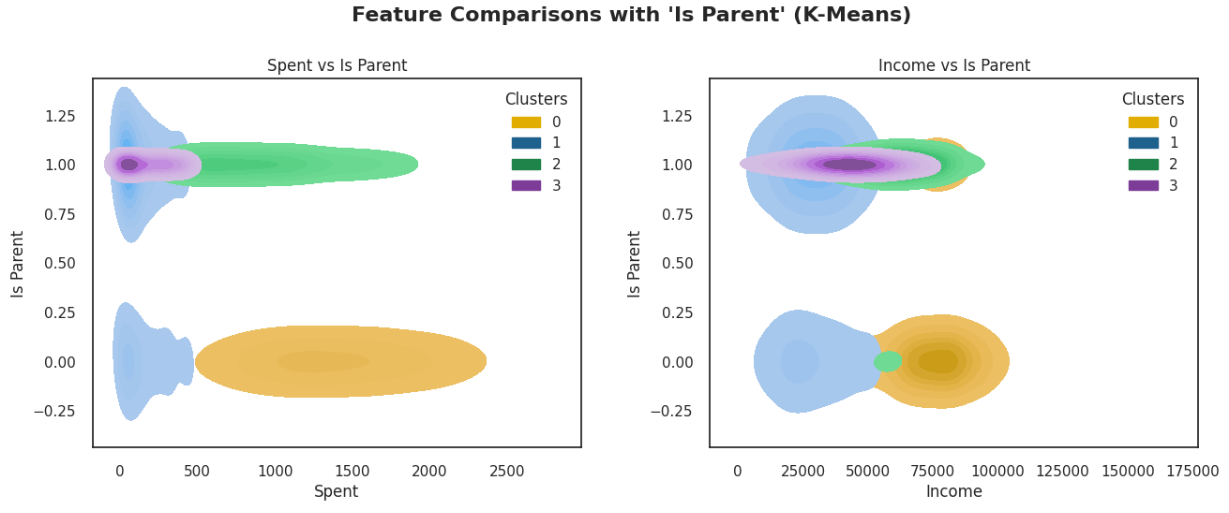
\includegraphics[width=15.25cm,height=6.36cm]{./images/image31.png}
\end{figure}


\textbf{Insights:} Using the previous chart \textit{Spent vs Is\_Parent} as a reference for comparison, we can see a pattern between parental spendings and income. As clearly established by previous charts, \uline{\textcolor[HTML]{BF9000}{Cluster 0}} has the highest income. However, the interesting discovery is the incomes of the parents. All clusters, except \uline{\textcolor[HTML]{BF9000}{Cluster 0}}, that are classified as parents generally experience an elevated income compared to their non-parental income. This is particularly true for \uline{\textcolor[HTML]{38761D}{Cluster 2}}\ \ and \uline{\textcolor[HTML]{674EA7}{Cluster 3}}, which previous charts identified as the most interested in parenting.

\vspace{1\baselineskip}
\textbf{Conclusions:} As the right sub-plot shows, combined with correlations involving previous charts, there is a general trend between an individual’s income and perspective on the topic of parenting. The more invested in parenting a group of individuals is, the higher their income becomes relative to their particular personality traits that limits their work ethic and potential to make more money. For instance, \uline{\textcolor[HTML]{BF9000}{Cluster 0}} may have the highest income and have a strong aversion toward starting a family, but their inherent personality traits promote a work ethic that drives them to work harder and make more money. In contrary, \uline{\textcolor[HTML]{38761D}{Cluster 2}} and \uline{\textcolor[HTML]{674EA7}{Cluster 3}} have personal preferences of investing time beyond work, which explains their low income relative to \uline{\textcolor[HTML]{BF9000}{Cluster 0}}, as shown in the \textit{Spending vs Income} chart at the beginning of the section ``Further Cluster Analysis of the Baseline method K-Means". However, in the chart above, it is evident that parents in \uline{\textcolor[HTML]{38761D}{Cluster 2}} and \uline{\textcolor[HTML]{674EA7}{Cluster 3}}, who predominantly choose to have children according to insights from previous charts, surpass their baseline income or lifestyle level upon being parents. Furthermore, \uline{\textcolor[HTML]{674EA7}{Cluster 3}}, the group with the lowest income, now surpasses \uline{\textcolor[HTML]{0B5394}{Cluster 1}} and comes close to matching the affluence of \uline{\textcolor[HTML]{38761D}{Cluster 2}}. Similarly, parents in \uline{\textcolor[HTML]{38761D}{Cluster 2}} nearly achieve the same income level as those in \uline{\textcolor[HTML]{BF9000}{Cluster 0}}.

\vspace{1\baselineskip}
\section{Business Impact}

The defined business objective, driven by the research question, was to develop clustering models that group the data and uncover insights from the resulting cluster structures. These insights are then analyzed and extended to broader contexts, such as spending patterns and personality traits, to reveal the unique characteristics of each segmented group. By leveraging this meaningful information, we can achieve actionable wisdom, using the segmentation to enable data-driven decision-making. A few key benefits include:

\begin{itemize}
	\item Targeting audiences more effectively based on marital status, parental status, age, income, and spending patterns

	\item Designing more impactful and efficient marketing campaigns

	\item Reducing wasted resources by avoiding outreach to audiences whose personalities don’t align with the intended message

\end{itemize}
\vspace{1\baselineskip}
Achieving these milestones require high-quality clusters that allow clear distinctions between segments, making it possible to identify meaningful patterns. To evaluate the quality of the clustering methods, the Silhouette Score metric from -1 to 1 was used. The results were as follows:

\begin{itemize}
	\item K-Means: 0.388 (69.4$\%$)

	\item Agglomerative Clustering: 0.348 (67.4$\%$)

	\item Spectral Clustering: 0.369 (68.45$\%$)

\end{itemize}
\vspace{1\baselineskip}
Among these methods, K-Means, which served as the baseline, achieved the highest Silhouette Score of 0.388, equating to 69.4$\%$. This indicates high-quality clusters with strong intra-cluster cohesion and low inter-cluster overlap. Agglomerative and Spectral Clustering also produced competitive results, with scores of 67.4$\%$ and 68.45$\%$. It’s important to note that these percentages don’t represent accuracy, as they do in classification tasks. Instead, they serve as indicators of how well the clusters are separated, providing a measure of their reliability for generating insights. Rather than reflecting "right" or "wrong" outcomes, these scores assess the clarity and trustworthiness of the visualized clusters for informed decision-making.

\vspace{1\baselineskip}
\subsection{Business Conclusions}

Now, once the clusters have been visualized and evaluated by their reliability, it’s time to make conclusions from the business and marketing perspective. The insights below represent the key findings which are valuable for stakeholders and managers to adjust or tailor marketing efforts. More precisely, this section uses the insights from the section ``3. Results $\&$ Conclusions" and concisely frames them in the light of the defined business objective:

\begin{table}[H]
\begin{adjustbox}{max width=\textwidth}
\begin{tabular}{p{1.98cm}p{2.17cm}p{2.59cm}p{1.93cm}p{2.51cm}p{2.99cm}p{1.98cm}p{2.17cm}p{2.59cm}p{1.93cm}p{2.51cm}p{2.99cm}}
\hline
\multicolumn{1}{|p{1.98cm}}{\centering
Cluster} & 
\multicolumn{1}{|p{2.17cm}}{\centering
Parent Status} & 
\multicolumn{1}{|p{2.59cm}}{\centering
Family Size} & 
\multicolumn{1}{|p{1.93cm}}{\centering
Income} & 
\multicolumn{1}{|p{2.51cm}}{\centering
Age Range} & 
\multicolumn{1}{|p{2.99cm}|}{\centering
Additional Notes} \\ 
\hline
\multicolumn{1}{|p{1.98cm}}{\centering
\uline{\textcolor[HTML]{BF9000}{Cluster 0}}} & 
\multicolumn{1}{|p{2.17cm}}{\centering
{\footnotesize Strong aversion to parenting}} & 
\multicolumn{1}{|p{2.59cm}}{\centering
{\footnotesize Alone or with one partner}} & 
\multicolumn{1}{|p{1.93cm}}{\centering
{\footnotesize High}} & 
\multicolumn{1}{|p{2.51cm}}{\centering
{\footnotesize Uniform distribution: 30-80}} & 
\multicolumn{1}{|p{2.99cm}|}{\centering
{\footnotesize Values quality over quantity}} \\ 
\hline
\multicolumn{1}{|p{1.98cm}}{\centering
\uline{\textcolor[HTML]{0B5394}{Cluster 1}}} & 
\multicolumn{1}{|p{2.17cm}}{\centering
{\footnotesize Majority are parents}} & 
\multicolumn{1}{|p{2.59cm}}{\centering
{\footnotesize Usually 1 kid}} & 
\multicolumn{1}{|p{1.93cm}}{\centering
{\footnotesize Low}} & 
\multicolumn{1}{|p{2.51cm}}{\centering
{\footnotesize Mostly 35-55}} & 
\multicolumn{1}{|p{2.99cm}|}{\centering
{\footnotesize Values durable and cost-effective products}} \\ 
\hline
\multicolumn{1}{|p{1.98cm}}{\centering
\uline{\textcolor[HTML]{38761D}{Cluster 2}}} & 
\multicolumn{1}{|p{2.17cm}}{\centering
{\footnotesize 100$\%$ parents}} & 
\multicolumn{1}{|p{2.59cm}}{\centering
{\footnotesize Usually 2 kids}} & 
\multicolumn{1}{|p{1.93cm}}{\centering
{\footnotesize High}} & 
\multicolumn{1}{|p{2.51cm}}{\centering
{\footnotesize Mostly 50-75}} & 
\multicolumn{1}{|p{2.99cm}|}{\centering
{\footnotesize Likes quality products and family product bundles}} \\ 
\hline
\multicolumn{1}{|p{1.98cm}}{\centering
\uline{\textcolor[HTML]{674EA7}{Cluster 3}}} & 
\multicolumn{1}{|p{2.17cm}}{\centering
{\footnotesize 100$\%$ parents}} & 
\multicolumn{1}{|p{2.59cm}}{\centering
{\footnotesize Usually 2-3 kids}} & 
\multicolumn{1}{|p{1.93cm}}{\centering
{\footnotesize Low}} & 
\multicolumn{1}{|p{2.51cm}}{\centering
{\footnotesize Mostly 50-75}} & 
\multicolumn{1}{|p{2.99cm}|}{\centering
{\footnotesize Prioritizes large product bundles for family needs}} \\ 
\hline
\end{tabular}
\end{adjustbox}
\end{table}
\vspace{5\baselineskip}

\textbf{Marketing of products}


\textit{The conclusions below are based on the insights of popularity of discount family deals, incomes, spendings, parental status and marital status}

\vspace{1\baselineskip}
\begin{itemize}
	\item \textbf{High parental investment:} Marketing efforts for families is more favorable for \uline{\textcolor[HTML]{674EA7}{Cluster 3}}, \uline{\textcolor[HTML]{0B5394}{Cluster 1}}, \uline{\textcolor[HTML]{38761D}{Cluster 2}}, and since \uline{\textcolor[HTML]{38761D}{Cluster 2}} has more disposable income, as a result of their higher education, they also tend to spend more money, making the return on investment in marketing campaign highest for targeting this cluster. However, since \uline{\textcolor[HTML]{674EA7}{Cluster 3}} has more kids, discount deals with more quantity of products targeting more persons or kids would entice \uline{\textcolor[HTML]{674EA7}{Cluster 3}}, since their main goal is to take care of all their kids while keeping their economy in check

\end{itemize}
\vspace{1\baselineskip}
\begin{itemize}
	\item \textbf{No parental investment:} In contrast, \uline{\textcolor[HTML]{BF9000}{Cluster 0}} that refrains from having kids is not ideal to target with these types of family-based discounts. Instead, they value quality over quantity, making premium deals a more suitable marketing appeal for them

\end{itemize}
\vspace{1\baselineskip}
\begin{itemize}
	\item \textbf{Moderate parental investment:} Also, \uline{\textcolor[HTML]{0B5394}{Cluster 1}} that sometimes have kids and sometimes not, coupled with their low income, find slightly more value in family discount deals, but what appeals to this group is mainly the practicality of the products. Instead of judging brands by their premium status as \uline{\textcolor[HTML]{BF9000}{Cluster 0}}, they primarily want the products they buy to work as intended for longer periods of time, saving them money

\end{itemize}
\vspace{1\baselineskip}
\section{Additional Configurations}

To begin, you need to select the number of clusters and a clustering method. While the default method for this project is K-Means, the notebook provides flexibility to switch to Spectral Clustering or Agglomerative Clustering. This can be done by simply updating the value of a specific variable. In the provided Python notebook, navigate to the section titled ``1.1 Developer’s Configurations". Here, you can modify two key variables:

\begin{itemize}
	\item \textit{selected\_clustering\_method:} Determines the clustering algorithm to be used. By changing its value, you can choose between K-Means, Spectral Clustering, or Agglomerative Clustering

	\item \textit{num\_clusters:} Specifies the number of clusters for the analysis

\end{itemize}
\vspace{1\baselineskip}
The sections below explain the impact of these variables on the results in greater detail.

\begin{figure}[H]
\centering
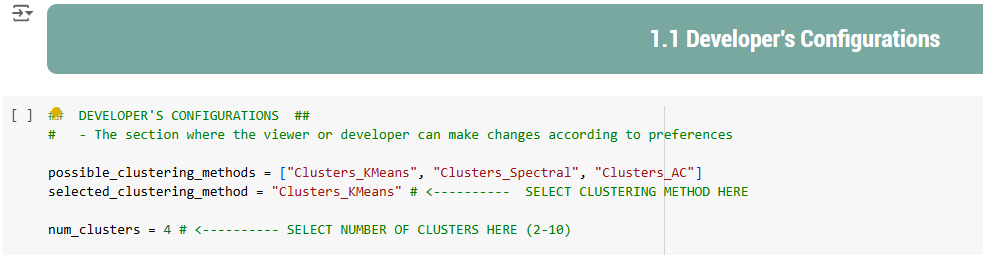
\includegraphics[width=15.49cm,height=4.01cm]{./images/image7.png}
\end{figure}


\vspace{1\baselineskip}
\subsection{Baseline Method Selection}

As established, the defined baseline method for this project report was K-Means. Nonetheless, the developer can easily alternate between Spectral and Agglomerative by simply changing the value of the variable \textit{selected\_clustering\_method}. To be clear, essentially what this does is to specify the method to use for further analysis and visualizations, once the summarized results of all three methods have been executed. In other words, the cluster formations and Silhouette scores of all three clustering methods shown in the section ``3.1 Multiple Cluster Method Comparison" are always executed, regardless of the selected baseline method. However, changing the value of \textit{selected\_clustering\_method} replaces the method used for further analysis and visualizations covered in the section ``3.2 Further Cluster Analysis of The Baseline Method". To switch between clustering methods, simply set the value of \textit{selected\_clustering\_method} to one of the options available in the list \textit{possible\_clustering\_methods}. While the overall cluster formations typically remain consistent across different methods, the colors assigned to each cluster may differ due to variations in the internal mechanics of the algorithms. Below are a few pictures generated when running the code with the two other methods configured as the baseline:

\vspace{1\baselineskip}
\ \ \ \uline{Spectral Clustering:}\ \ \ \ \ \ \ \ \ \ \ \ \ \ \ \ \ \ \ \ \uline{Agglomerative Clustering:}

\vspace{1\baselineskip}
\begin{figure}[H]
\centering
\begin{subfigure}[b]{0.45\textwidth}
\centering
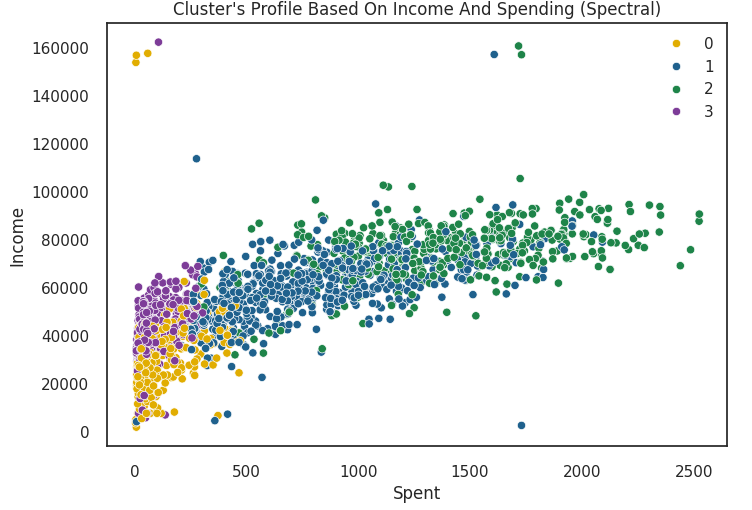
\includegraphics[width=\textwidth]{./images/image14.png}
\end{subfigure}
\hfill
\begin{subfigure}[b]{0.45\textwidth}
\centering
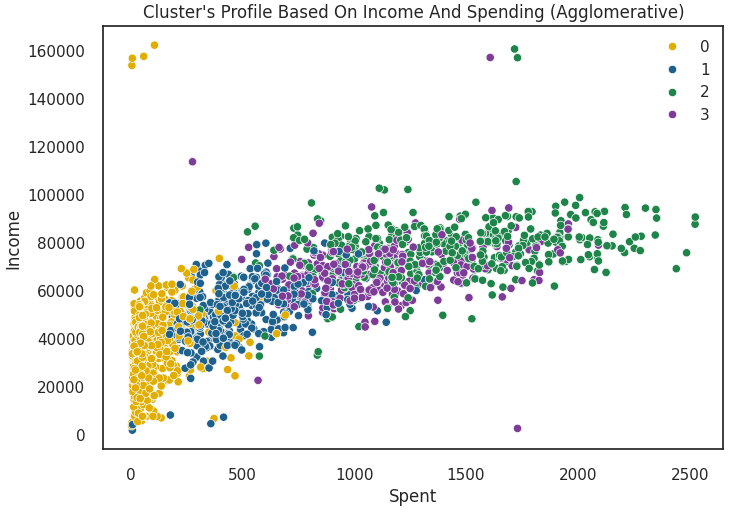
\includegraphics[width=\textwidth]{./images/image5.png}
\end{subfigure}
\end{figure}


\vspace{1\baselineskip}
\begin{figure}[H]
\centering
\begin{subfigure}[b]{0.45\textwidth}
\centering
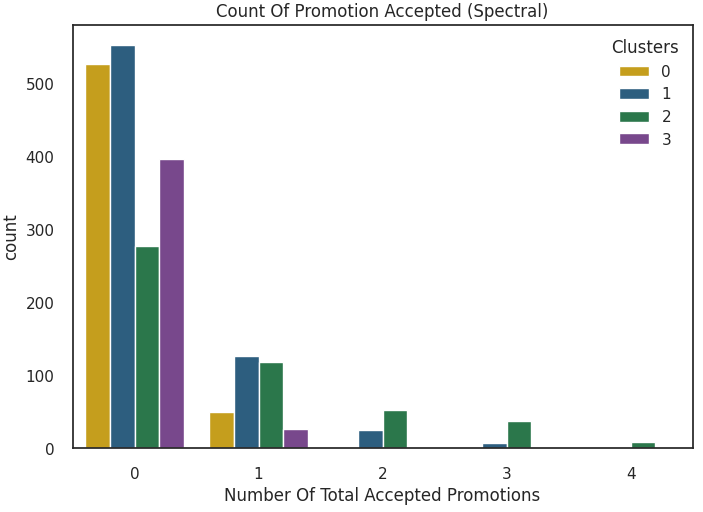
\includegraphics[width=\textwidth]{./images/image9.png}
\end{subfigure}
\hfill
\begin{subfigure}[b]{0.45\textwidth}
\centering
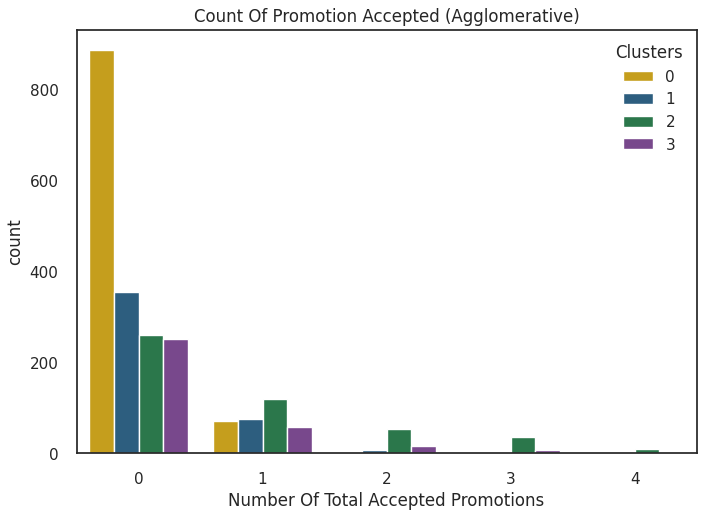
\includegraphics[width=\textwidth]{./images/image20.png}
\end{subfigure}
\end{figure}


\vspace{1\baselineskip}
\subsection{Number of Clusters Selection}

In this report, four clusters were used to segment individuals into distinct groups. However, the Python notebook code supports clustering with 2 to 10 groups. For the specific business objective of this project, four clusters provided an optimal balance between simplicity and accuracy, enabling clear and actionable insights into the differences among the segments. If the project's objectives or requirements change, or if future challenges necessitate a deeper analysis with more detailed distinctions, the number of clusters can be adjusted accordingly. This flexibility allows the corporation to align the clustering approach with evolving research questions, facilitating the extraction of meaningful insights and supporting data-driven decision-making. Ultimately, this adaptability enhances both business strategies and marketing efforts by leveraging behavioral insights effectively. Below, a few visualizations from executions of the notebook with different configurations of \textit{num\_clusters} is displayed to demonstrate the added flexibility that this implementation brings:

\vspace{1\baselineskip}
\begin{center}
\textbf{\textit{num\_clusters $=$ 2:}}
\end{center}


\vspace{1\baselineskip}
\begin{figure}[H]
\centering
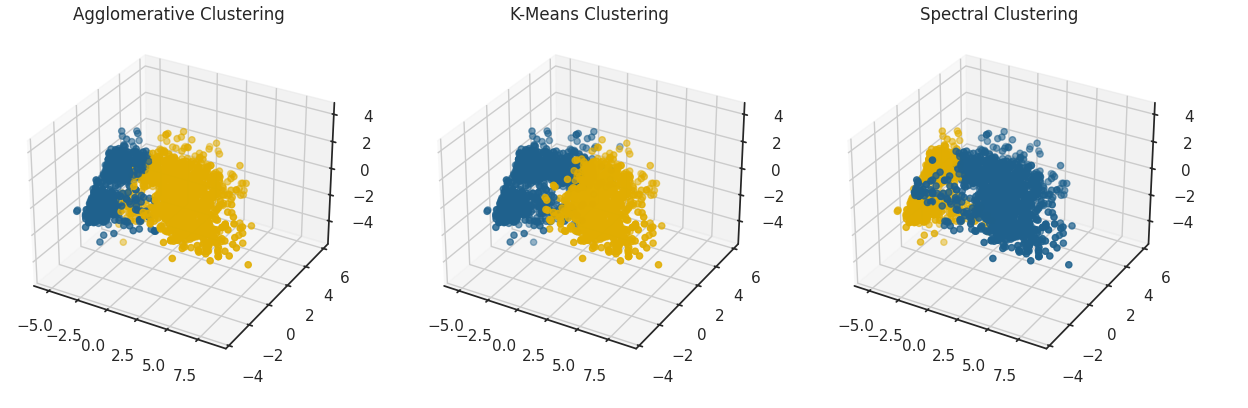
\includegraphics[width=14.41cm,height=4.72cm]{./images/image30.png}
\end{figure}


\vspace{3\baselineskip}
\begin{figure}[H]
\centering
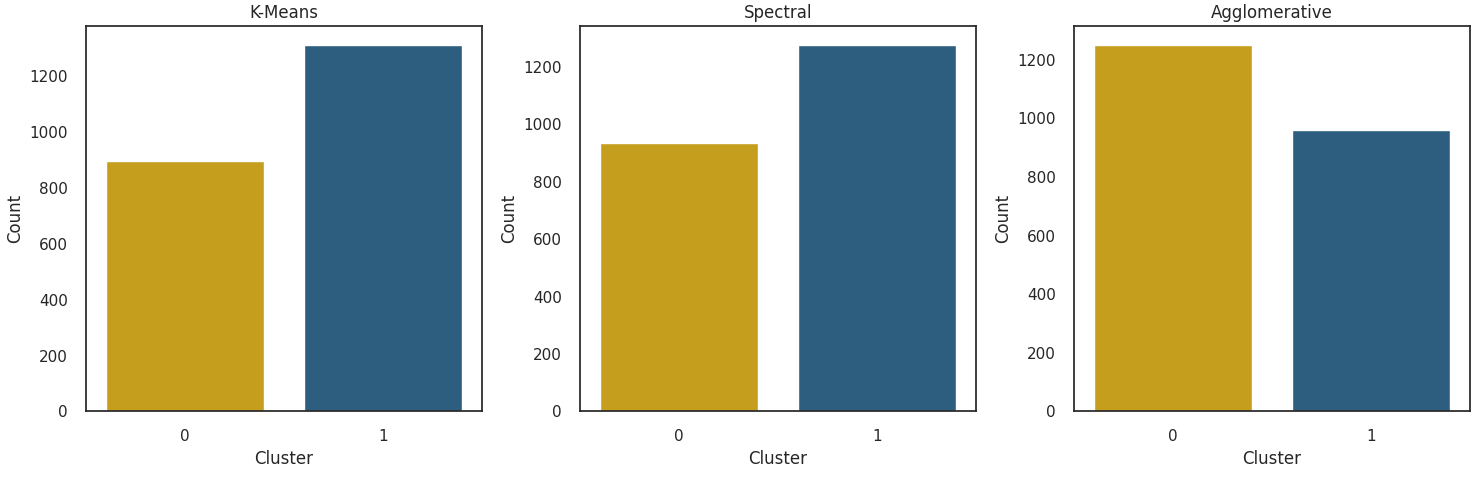
\includegraphics[width=14.06cm,height=4.56cm]{./images/image26.png}
\end{figure}


\begin{figure}[H]
\centering
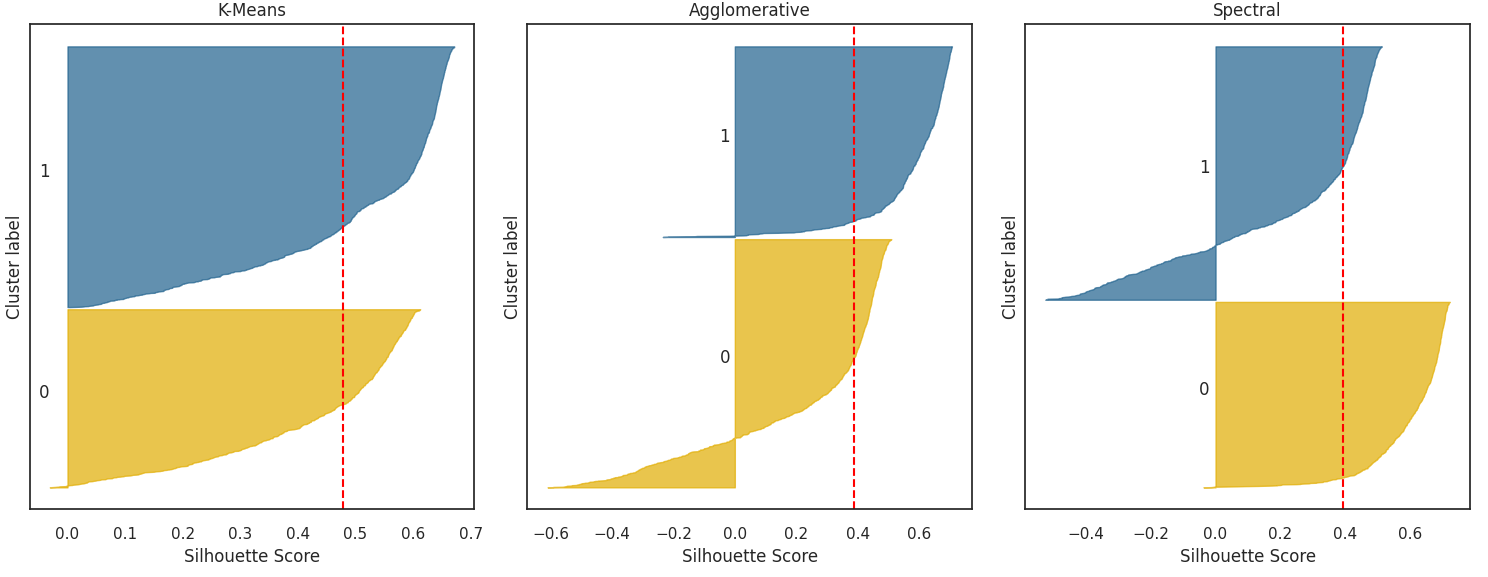
\includegraphics[width=13.43cm,height=5.2cm]{./images/image18.png}
\end{figure}


\begin{figure}[H]
\centering
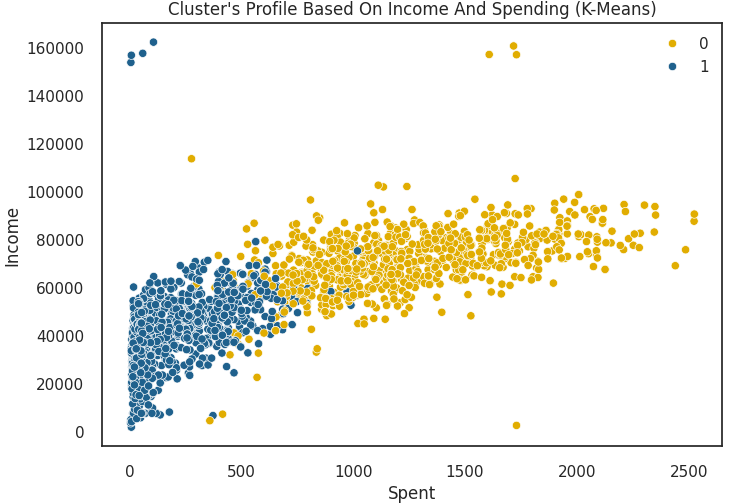
\includegraphics[width=10.7cm,height=7.26cm]{./images/image28.png}
\end{figure}


\vspace{3\baselineskip}
\begin{center}
\textbf{\textit{num\_clusters $=$ 6:}}
\end{center}


\vspace{1\baselineskip}
\begin{figure}[H]
\centering
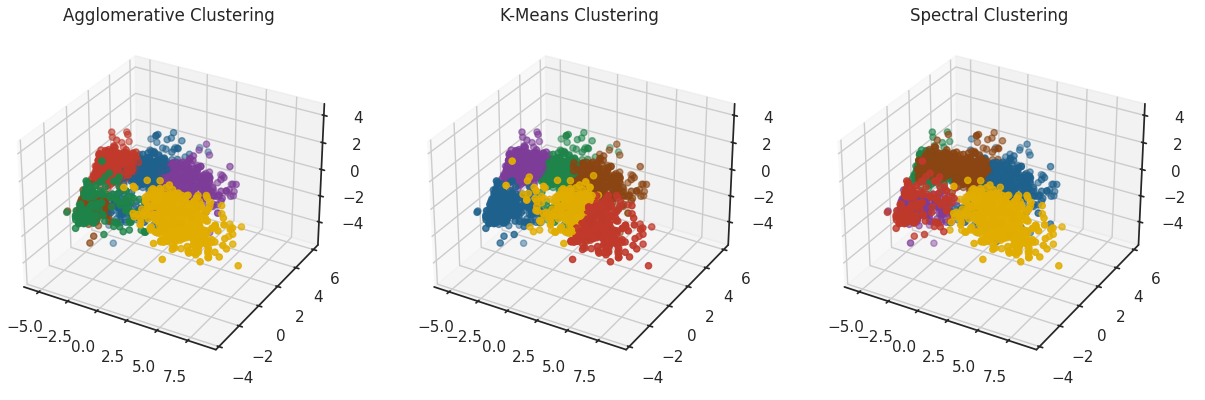
\includegraphics[width=15.92cm,height=5.29cm]{./images/image8.png}
\end{figure}


\begin{figure}[H]
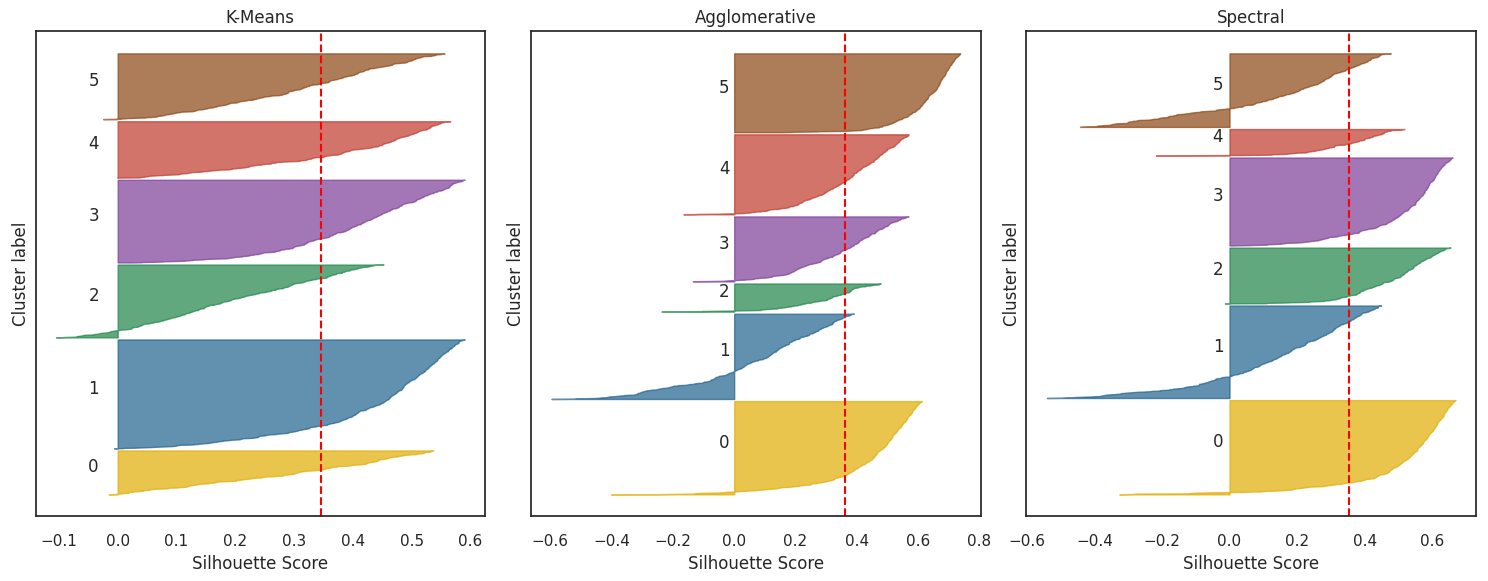
\includegraphics[width=14.59cm,height=5.7cm]{./images/image35.png}
\end{figure}


\begin{figure}[H]
\centering
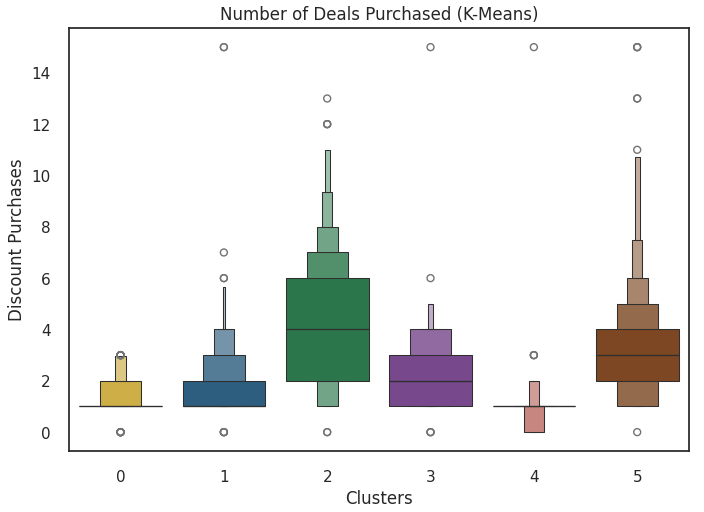
\includegraphics[width=10.42cm,height=7.55cm]{./images/image10.png}
\end{figure}


\vspace{2\baselineskip}
\begin{center}
\textbf{\textit{num\_clusters $=$ 10:}}
\end{center}


\vspace{1\baselineskip}
\begin{figure}[H]
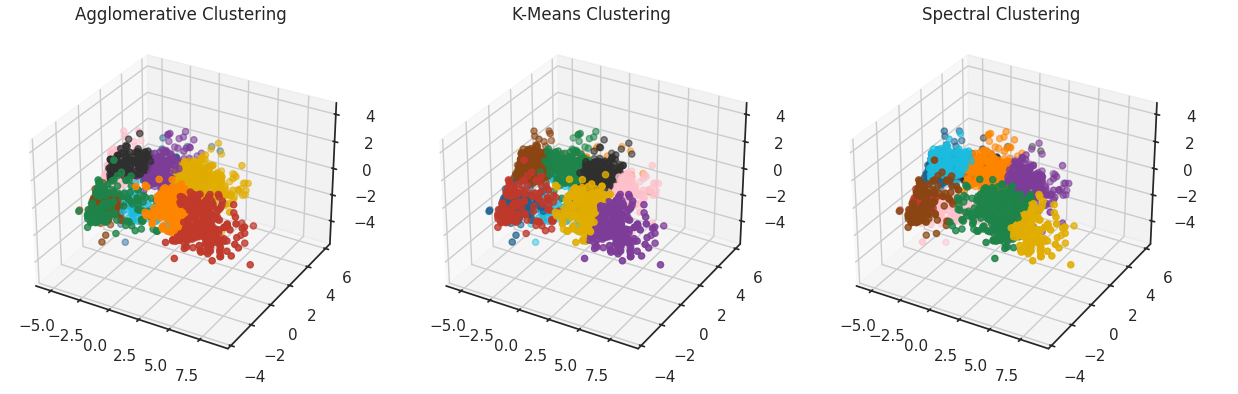
\includegraphics[width=15.92cm,height=5.08cm]{./images/image27.png}
\end{figure}


\begin{figure}[H]
\centering
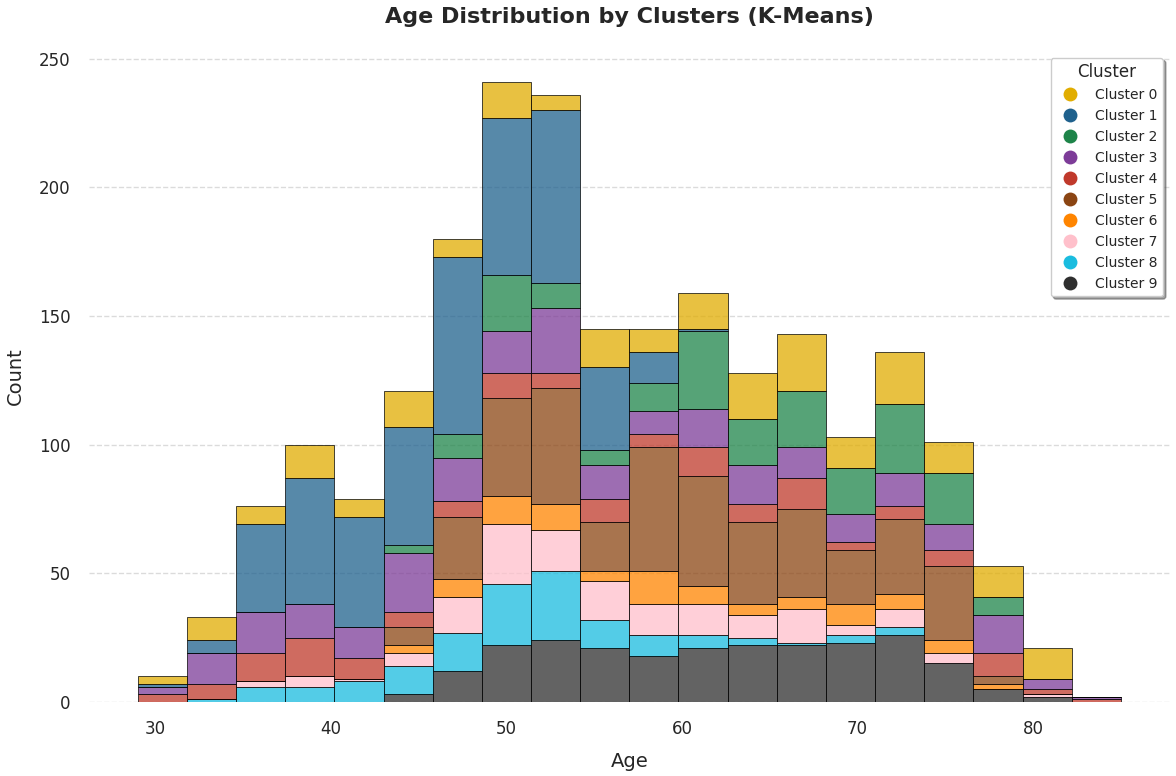
\includegraphics[width=13.61cm,height=8.98cm]{./images/image22.png}
\end{figure}



\end{document}